\documentclass[english]{article}
\usepackage[english]{babel} 
\usepackage[T1]{fontenc}
\usepackage[utf8x]{inputenc}
\usepackage{float}
\usepackage{graphicx}
\usepackage{hyperref}


\makeatletter
\usepackage[a4paper,top=2cm,bottom=2cm,left=2cm,right=2cm]{geometry}
\usepackage{enumitem}
\usepackage{subfig}
\usepackage{amsthm}
\usepackage{amsmath}
\usepackage{epstopdf}
\usepackage{fancyhdr}
\usepackage{booktabs,array}

\hyphenation{english}
\makeatother

\usepackage{babel}


\usepackage{listings}
\usepackage{xcolor} % for setting colors

% set the default code style
\lstset{
    frame=tb, % draw a frame at the top and bottom of the code block
    tabsize=4, % tab space width
    showstringspaces=false, % don't mark spaces in strings
    numbers=left, % display line numbers on the left
    commentstyle=\color{gray}, % comment color
    keywordstyle=\color{blue}, % keyword color
    stringstyle=\color{red} % string color
}


\begin{document}
\begin{titlepage}

	\begin{center}
		\begin{Large} \textbf{UNIVERSITY OF PADOVA} \\
		\end{Large} \vspace{1cm}
		\vspace{3cm}
		\begin{Large} Computer Vision \end{Large}
		\par\end{center}

	\begin{center}
		\begin{Large}Intermediate project report\\
		\end{Large}
		\par\end{center}

	\begin{center}
		\vspace{2cm}
		\begin{figure}[!htb]
			\centering 
\includegraphics[width=8cm]{figures/unipd-logo.png}\\

		\end{figure}

		\par\end{center}

	\begin{center}
		\vspace{2cm}
		\begin{Large} Marek Tatýrek  \\
					Mateusz Miroslaw Lis \\
		\end{Large} \vspace{2cm}
		\begin{Large} Academic Year 2024-2025 \end{Large}
		\par\end{center}
		
	\end{titlepage}
	
\tableofcontents
\newpage

\section{Introduction}

\subsection{Notes}
To make code more clear, we use:
\begin{itemize}
	\item \texttt{snake\_case} for variables
	\item \texttt{PascalCase} for classes
	\item \texttt{camelCase} for functions
\end{itemize}

\section{Overview}
\paragraph{}
We decided to use class design, where classes are logicaly separated depending on task.
Dataflow between classes is provided by several user structures. Data are processed squentialy.
Unfortunately used dataflow is not that clear because we havent been able to fully follow originally defined structure.
We also used Doxygen documentation so for detailed description you can check it \href{run:../latex/refman.pdf}{here}.
\paragraph{}
	For loading data we have two classes \texttt{ImageLoader()} and \texttt{VideoLoader()}, derived from class \texttt{InputSource()}.
	From user side the classes have common interface and usage is the same. Important is method \texttt{hasNextFrame()}, used for
	driving the while loop in the main, returning true in case there is frame or image that we can read. Class is returning timestamp,
	cv::Mat with current sample.

\paragraph{}
	As was already said, tasks are performed sequentialy, which is convenient, because we are reading many frames and to store them in the buffer,
	it will be very memory demanding. Also from the same reason we have to take care about not making deep copies.
\paragraph{}
	We have \texttt{Preprocessing()} class, for editing the image before actual detection of haar features.
\paragraph{}
	For detecting features in the images we are using class \texttt{HaarDetector()} using haar cascades for finding desired 
	patterns in the images. In our case faces and eyes.
\paragraph{}
	From the detected features we need to make evaluation and decide which shot type are we having. For this purpouse we have
	class \texttt{FeatureEvaluator()} that outputs structure \texttt{classification\_result} with information if is curent sample
	wide shot, medium or close up.
\paragraph{}
	Because we want to make statictic from the data, we made \texttt{FilmStatistics()} class. It makes sense to use this class only on
	video data. At the init we provide configuration structure \texttt{FilmStatisticsEvalConfig}, with many settings. 
	We can export time sequences to \texttt{.csv} file or we can use getters to get the time sequences and use them in the code.
\paragraph{}
	For graphical output of the statstic data we have \texttt{ResultDisplayer()} class, which is inputting all data types got
	from \texttt{FilmStatistics()} getters and returning \texttt{cv::mat} with plots.

\section{Implementation details}

	\subsection{FileLoader}
		In this file we have four classes.
		\paragraph{}
			Class \texttt{InputSource} is parent class for \texttt{ImageLoader}
			and \texttt{VideoLoader} It serves to provide easy interface to work with image and video files.
			In both cases we aiming to process data in series, that means frame by frame. 
			Both of these classes have same user interface made of:
			\begin{itemize}
				\item \texttt{hasNextFrame()} - returns if there is one more frame to process, used for driving while loop.
				\item \texttt{nextFrame()} - returns next frame in the sequence.
				\item \texttt{getCurrentTimestamp}() - returns current timestamp in ms.
			\end{itemize}
		\paragraph{}
			For preprocessing we have class \texttt{Preprocessing()}. We only implemented processing methods that we found 
			beneficial. The class contains this methods:
			\begin{itemize}
				\item \texttt{LoadFrame()}
				\item \texttt{resizeImage()}
				\item \texttt{toGrayscale()}
				\item \texttt{equalizeHistogram()}
				\item \texttt{GetProcessedImage()}
			\end{itemize}
			Names on methods are describing function sufficiently.

	\subsection{SceneChangeDetect} \label{optimizer}
		\paragraph{}
			This file contains single function for optimizing processing of Viola \& Johnes detector.
			As an input we take two frames, we compute how much they are different and return boolean value.
			Because Viola \& Johnes is computationaly quite expansive, we want to proccess the frame by it, only when it is really 
			needed.
			
		\paragraph{}
			We have two parameters:
			\begin{itemize}
				\item \texttt{pixelDiffThreshold} - Difference between two pixel at same position in input frames.
				\item \texttt{threshold} - Percentage of pixels, that reach \texttt{pixelDiffThreshold} parameter value.
			\end{itemize}
		\paragraph{}
			Algorithm computes difference between all pixel at apropriate positions and make boolean array. Then 
			it computes percetage of pixels that reaches the \texttt{pixelDiffThreshold} and compare the value with \texttt{threshold}.
			If the computed value reaches the treshold it returns true.
			
	%...

	\subsection{TestDatasetEval}
		\paragraph{}
			This simple class is designed for computing accuracy of the algorithm on the test dataset. That means at image dataset.
			Since we have test datased sorted in the folders, task is pretty simple. We have class \texttt{TestDatasetEval}.
			with constructor we pass \texttt{ShotType}, which we want to test with this class. Then we have two methods:
			\begin{itemize}
				\item \texttt{check()} Is used in while to add currently classified image ShotType to evaluation.
				\item \texttt{getEvalResults()} After all images are processed we call this method and it returns accuracy.
			\end{itemize}

	\subsection{FilmStatistics} \label{filmstats}
		\paragraph{}
			Class is mainly designed for video. As input it takes class probabilities and it outputs \texttt{.csv} file with
			statictical data. Constructor takes one argument - structure \texttt{FilmStatisticsEvalConfig}, which is used to set up all the parameters
			for class.

		\paragraph{}
			We have 4 public methods:
			\begin{itemize}
				\item \texttt{addConfigurationStruct()} - Serves to change configuration setings.
				\item \texttt{addFrameResult()} - Add frame to final evaluation.
				\item \texttt{exportToCSV()} - Exports computed statistical timelines to \texttt{csv} file for future processing.
				\item \texttt{printSummary()} - Prints basic statistical summary.
			\end{itemize}

		\paragraph{}
			It is important to mention what specificaly class does. It takes input probability. We can set oversapling or skipping to
			input data to filter random noise etc. Class computes entropy and entropy variance, it detects cuts in the scenes
			and clasify most probable \texttt{ShotType}. We can set different window sizes for oversampling window, entropy window and 
			entropy variance window. We can also reduce output data flow if we dont want to have informations from each single shot and we reduce size
			of output \texttt{csv} file. All of these parameters are settable in \texttt{FilmStatisticsEvalConfig}.
		\paragraph{}
			Since we are using sliding windows for signal processing, we introduce delay to the system, which grows as
			we setting bigger window sizes. Delay is different for each statistical parameter timeseries. Class handle this situation and starts
			outputing data when all of the parameters are valid, with correct timestamp.

	\subsection{Main video}
		\paragraph{}
			Puropuse of this main is to classify video. At first we initialize all the classes and time measurements.
			Then we run main while loop, until we run out of frames. We can see the main loop on scheme \ref{fig:video_main}

					\begin{figure}[H]
			\centering
			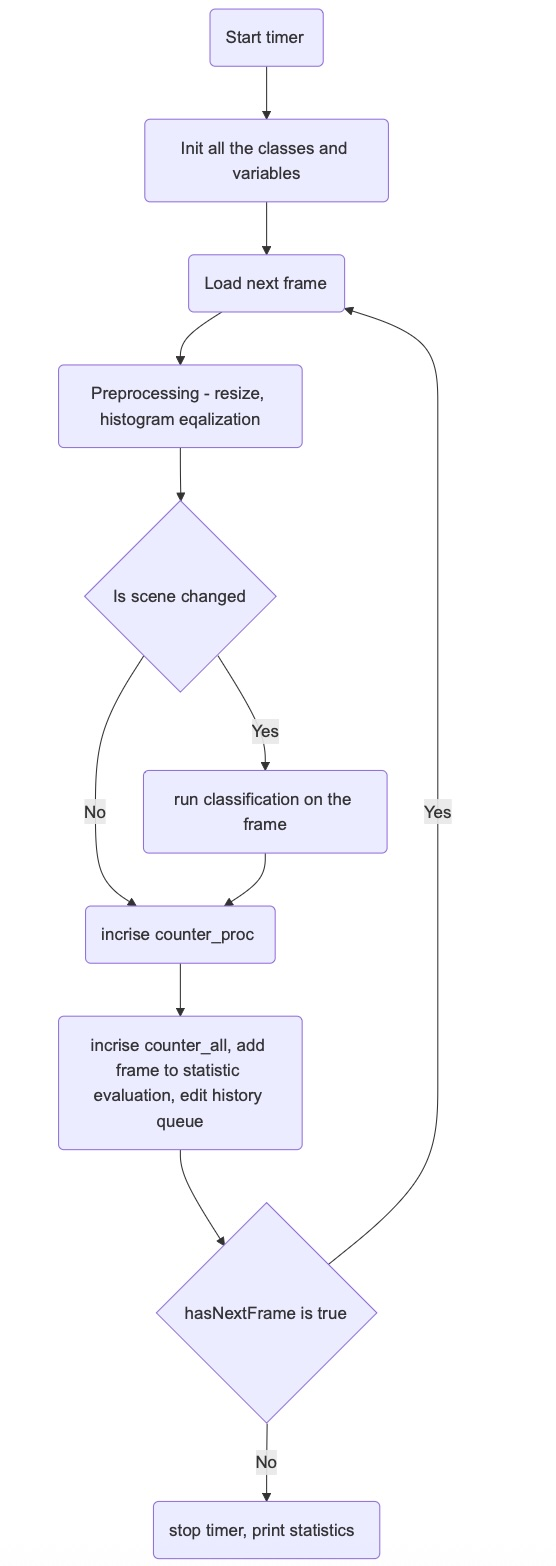
\includegraphics[width=0.5\textwidth]{figures/video_main_scheme.jpg}
			\caption{Classification with Viola\&Johnes}
			\label{fig:video_main}
		\end{figure}

	\section{Evaluation}
		\subsection{Quantitative Evaluation}
			Evaluating our classifier system on the test dataset can be done by running \texttt{main\_eval.cpp} from the submitted archive. Evaluation is done by computing one-vs-all precision, recall, F1 score, accuracy and the confusion matrix.


			\begin{table}[h!]
			\centering
				\begin{tabular}{|l|c|c|c|c|}
					\hline
						\textbf{Shot Type} & \textbf{Precision} & \textbf{Recall} & \textbf{F1 Score} & \textbf{Accuracy} \\
						\hline
						Close-up & 0.8889 & 0.8000 & 0.8421 & 0.9000 \\
						Medium   & 0.8000 & 0.8000 & 0.8000 & 0.8667 \\
						Wide     & 0.7273 & 0.8000 & 0.7619 & 0.8333 \\
					\hline
				\end{tabular}
				\caption{Per-class performance metrics for shot type classification}
			\end{table}

		\noindent\textbf{Overall Accuracy:} 0.8000

		\vspace{1em}

			\begin{table}[h!]
				\centering
					\begin{tabular}{|l|c|c|c|}
						\hline
							\textbf{Actual \textbackslash\ Predicted} & \textbf{Close-up} & \textbf{Medium} & \textbf{Wide} \\
							\hline
							Close-up & 8 & 0 & 2 \\
							Medium   & 1 & 8 & 1 \\
							Wide     & 0 & 2 & 8 \\
						\hline
					\end{tabular}
				\caption{Confusion matrix of the shot type classifier}
			\end{table}

	

		\subsubsection{Close up shots}
        \begin{figure}[H]
            \centering

            \subfloat[CLOSE\_UP]{%
                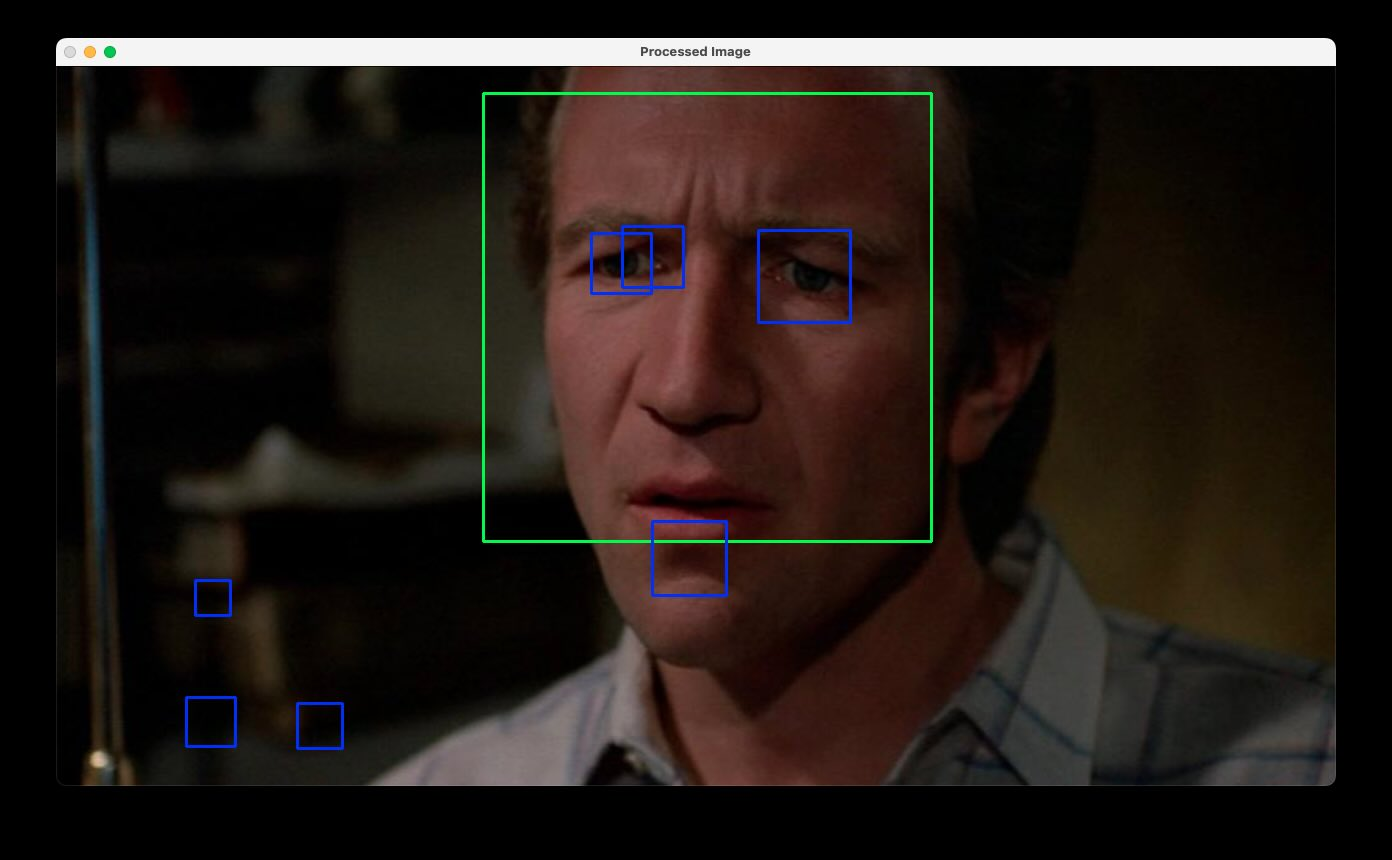
\includegraphics[width=0.32\textwidth]{result_images/closeup/ss1}
            }
            \hfill
            \subfloat[CLOSE\_UP]{%
                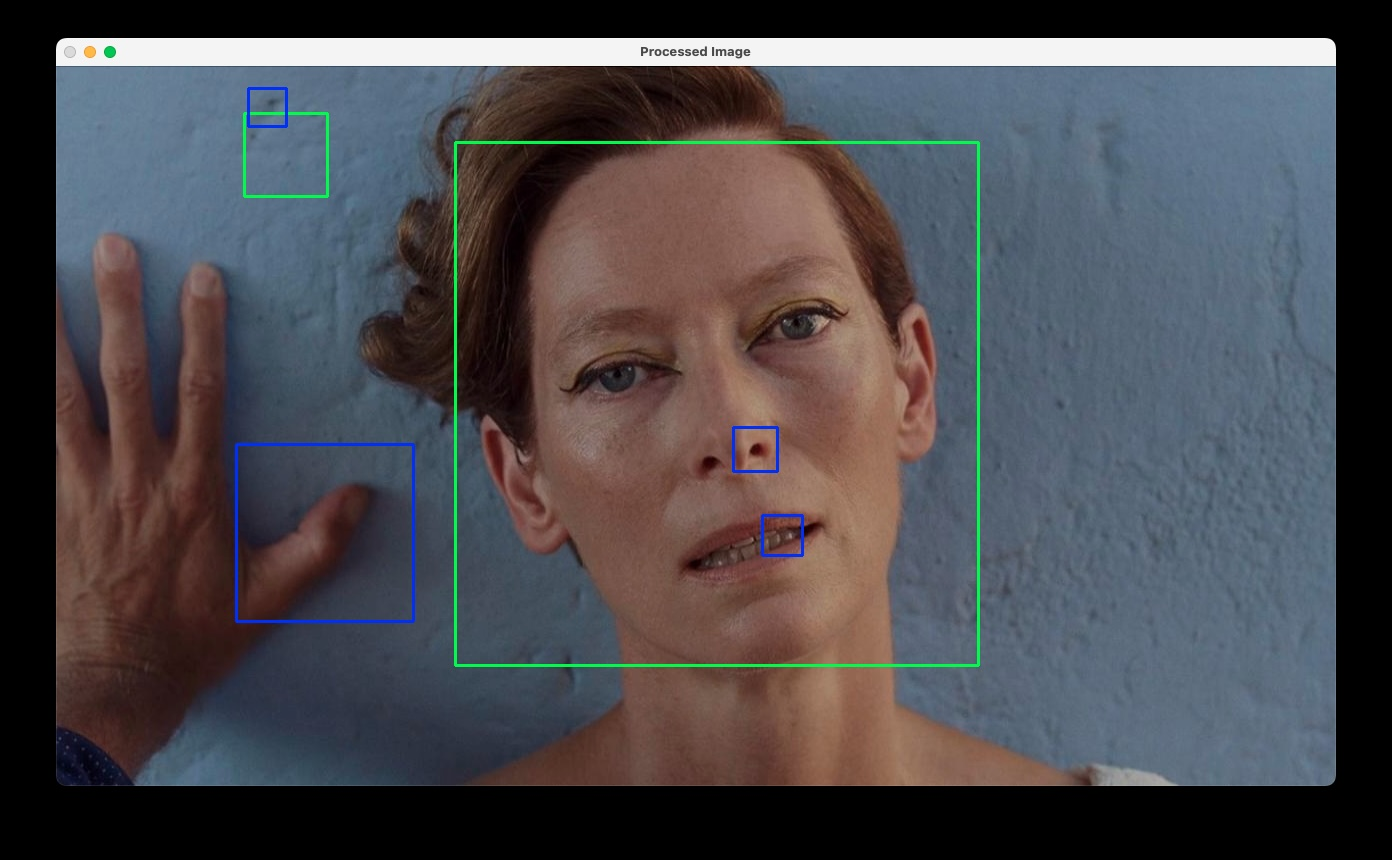
\includegraphics[width=0.32\textwidth]{result_images/closeup/ss2}
            }
            \hfill
            \subfloat[CLOSE\_UP]{%
                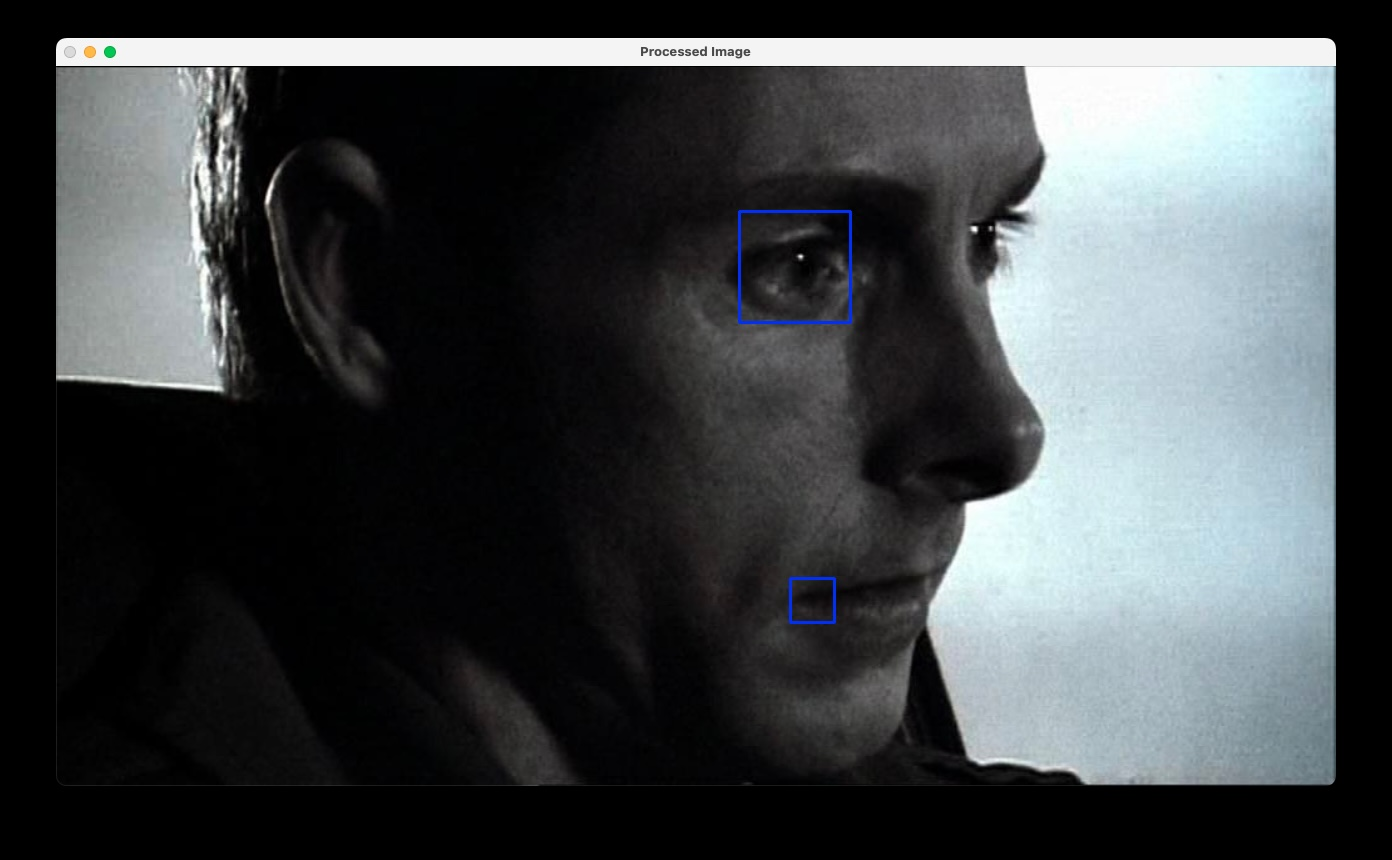
\includegraphics[width=0.32\textwidth]{result_images/closeup/ss3}
            }

            \vspace{1em}

            \subfloat[CLOSE\_UP]{%
                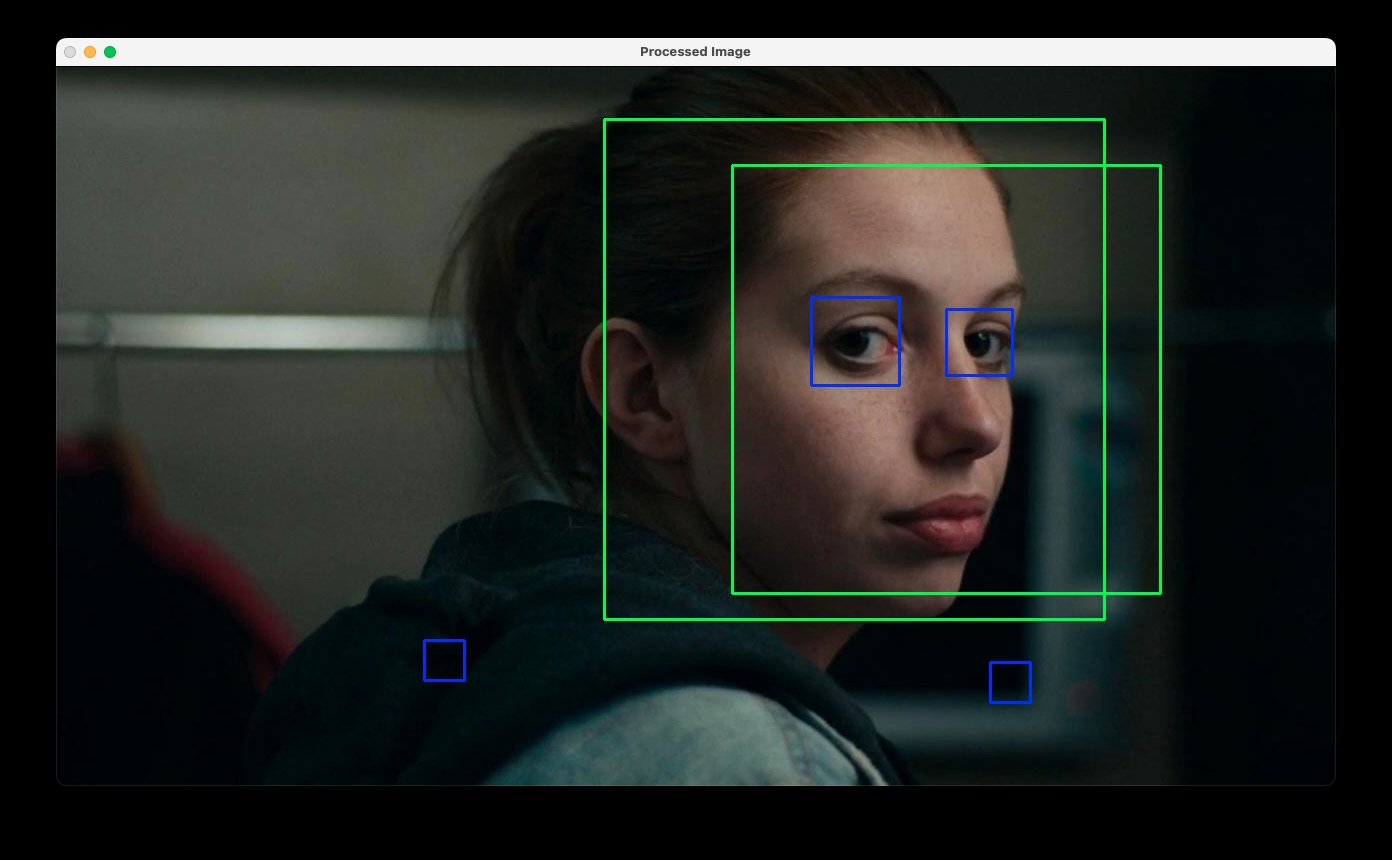
\includegraphics[width=0.32\textwidth]{result_images/closeup/ss4}
            }
            \hfill
            \subfloat[CLOSE\_UP]{%
                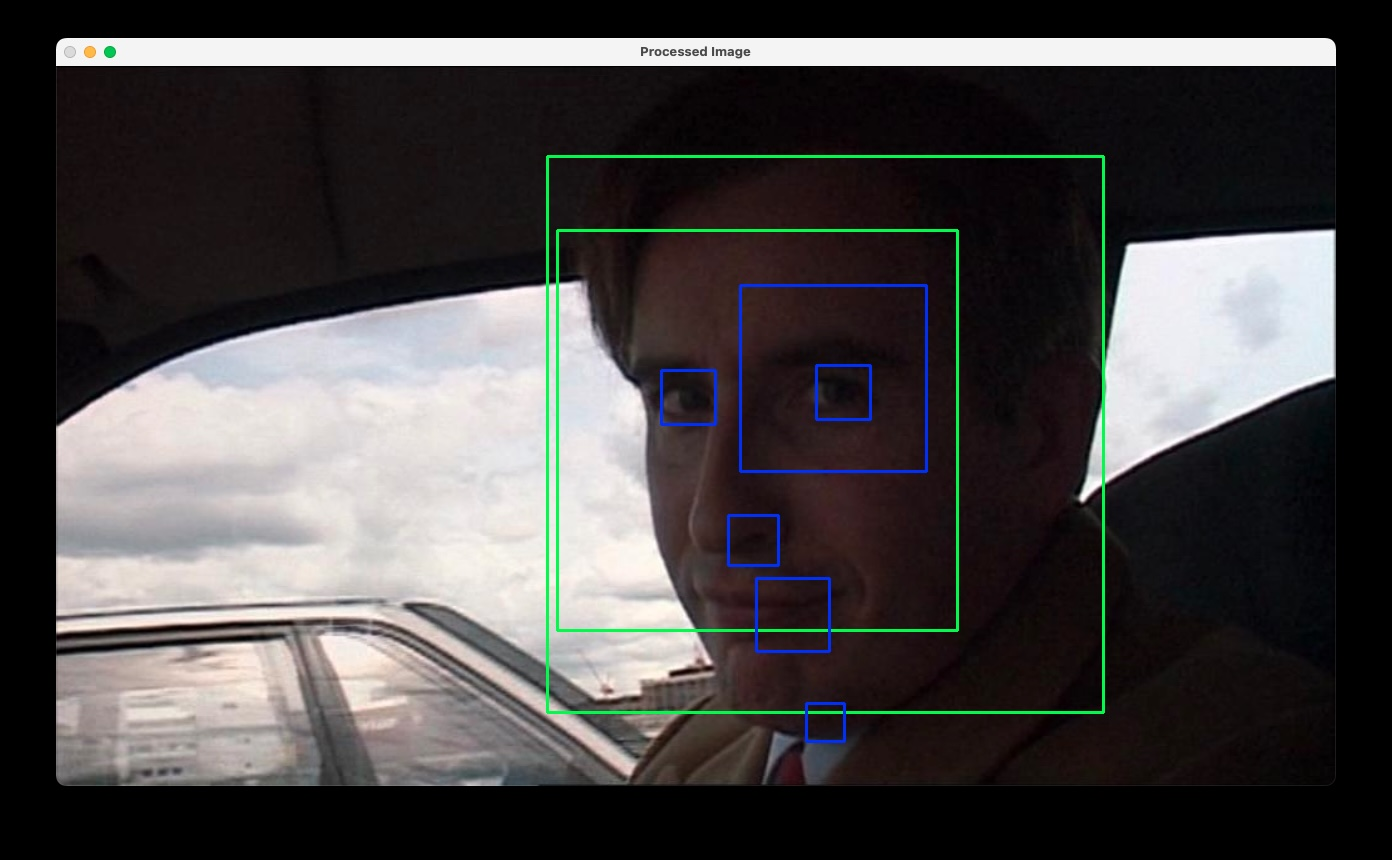
\includegraphics[width=0.32\textwidth]{result_images/closeup/ss5}
            }
            \hfill
            \subfloat[WIDE]{%
                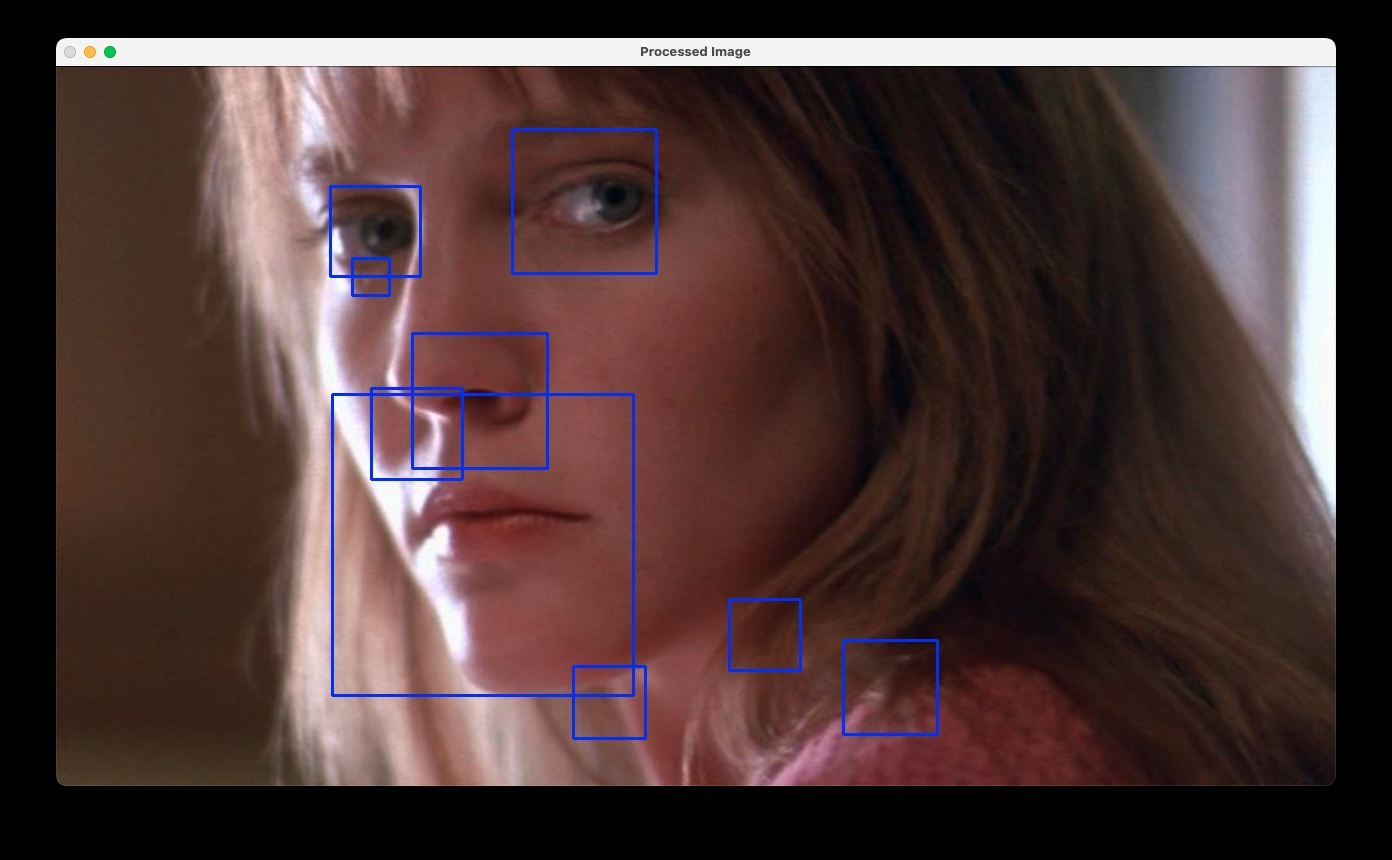
\includegraphics[width=0.32\textwidth]{result_images/closeup/ss6}
            }

            \vspace{1em}

            \subfloat[CLOSE\_UP]{%
                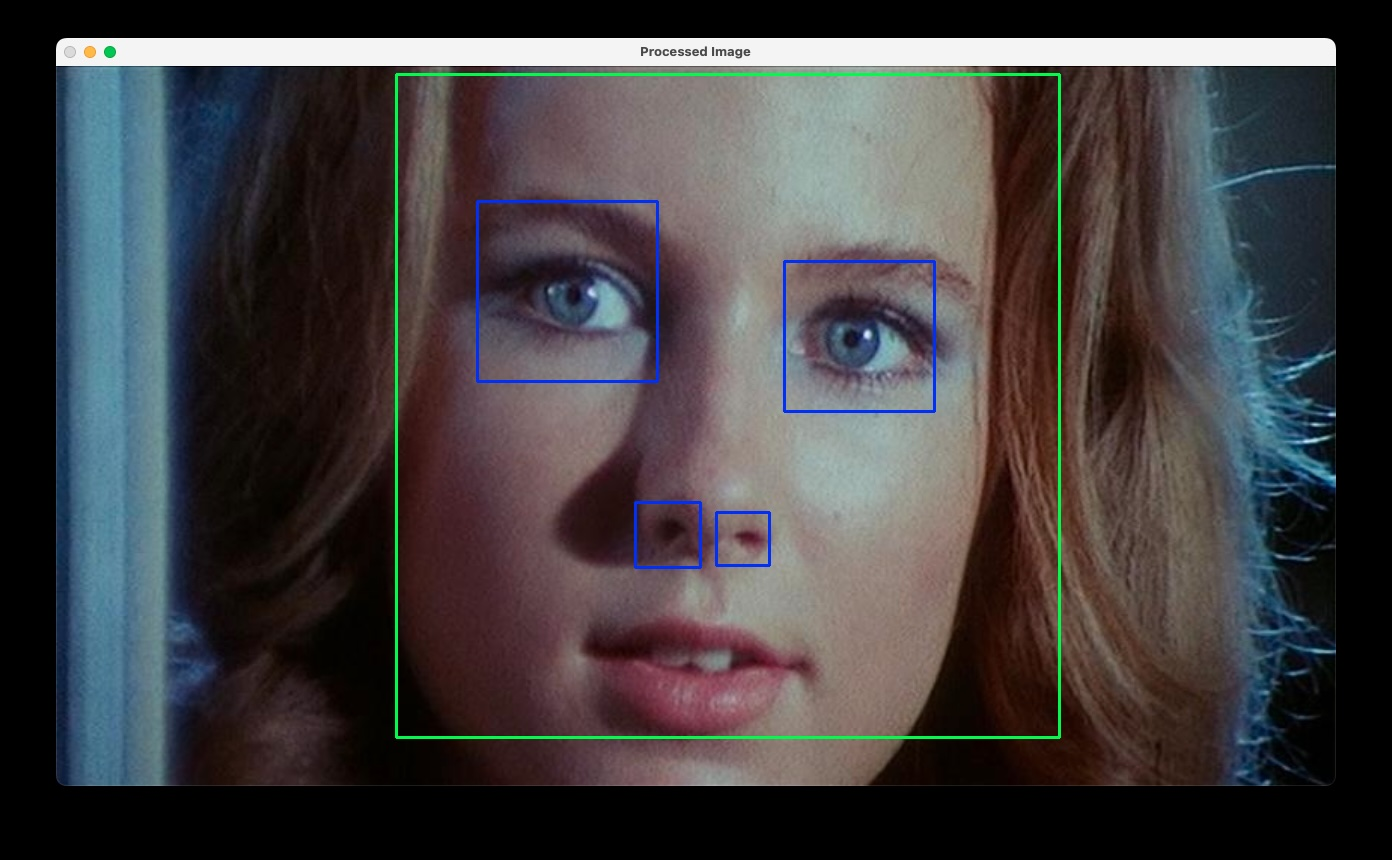
\includegraphics[width=0.32\textwidth]{result_images/closeup/ss7}
            }
            \hfill
            \subfloat[CLOSE\_UP]{%
                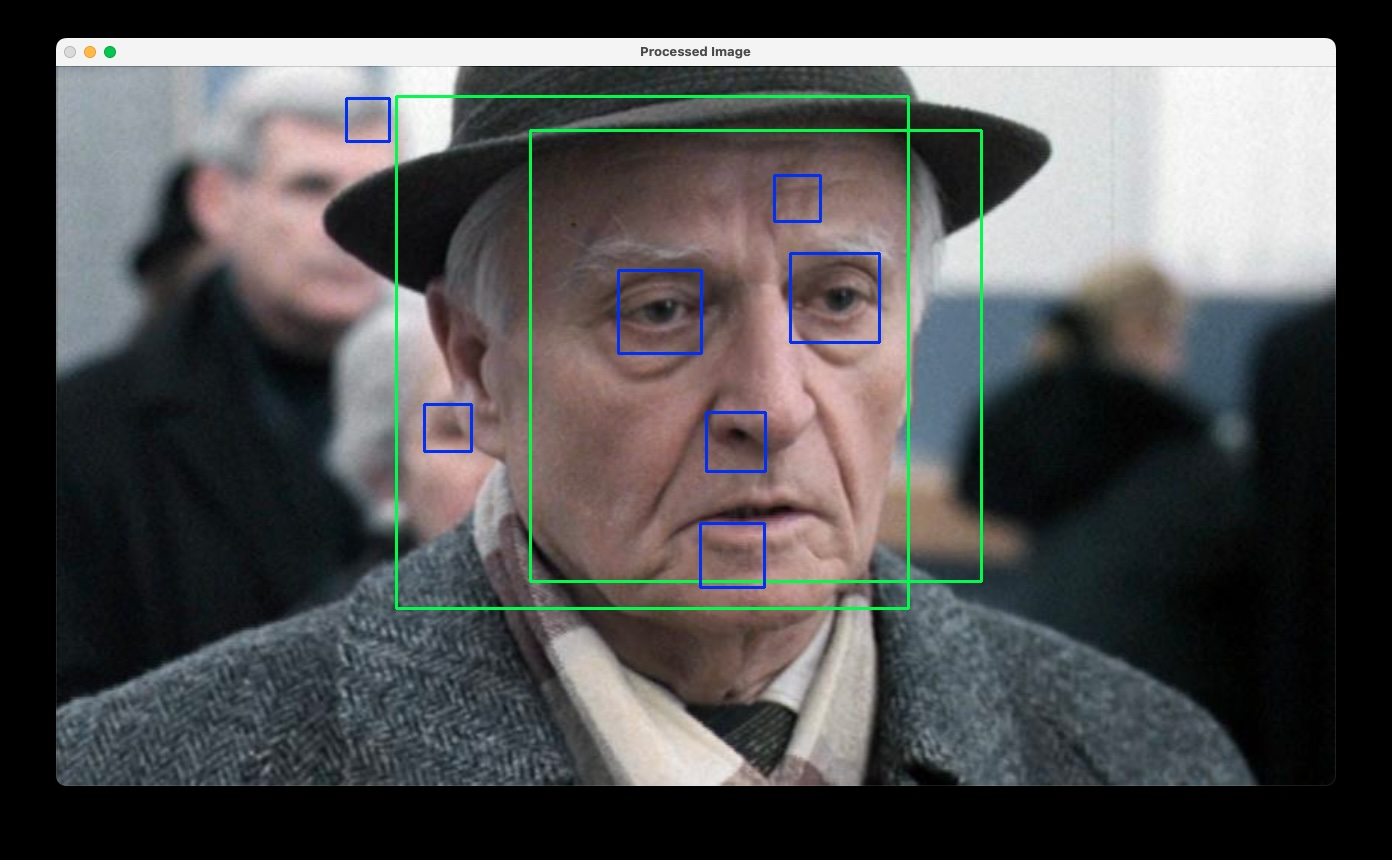
\includegraphics[width=0.32\textwidth]{result_images/closeup/ss8}
            }
            \hfill
            \subfloat[CLOSE\_UP]{%
                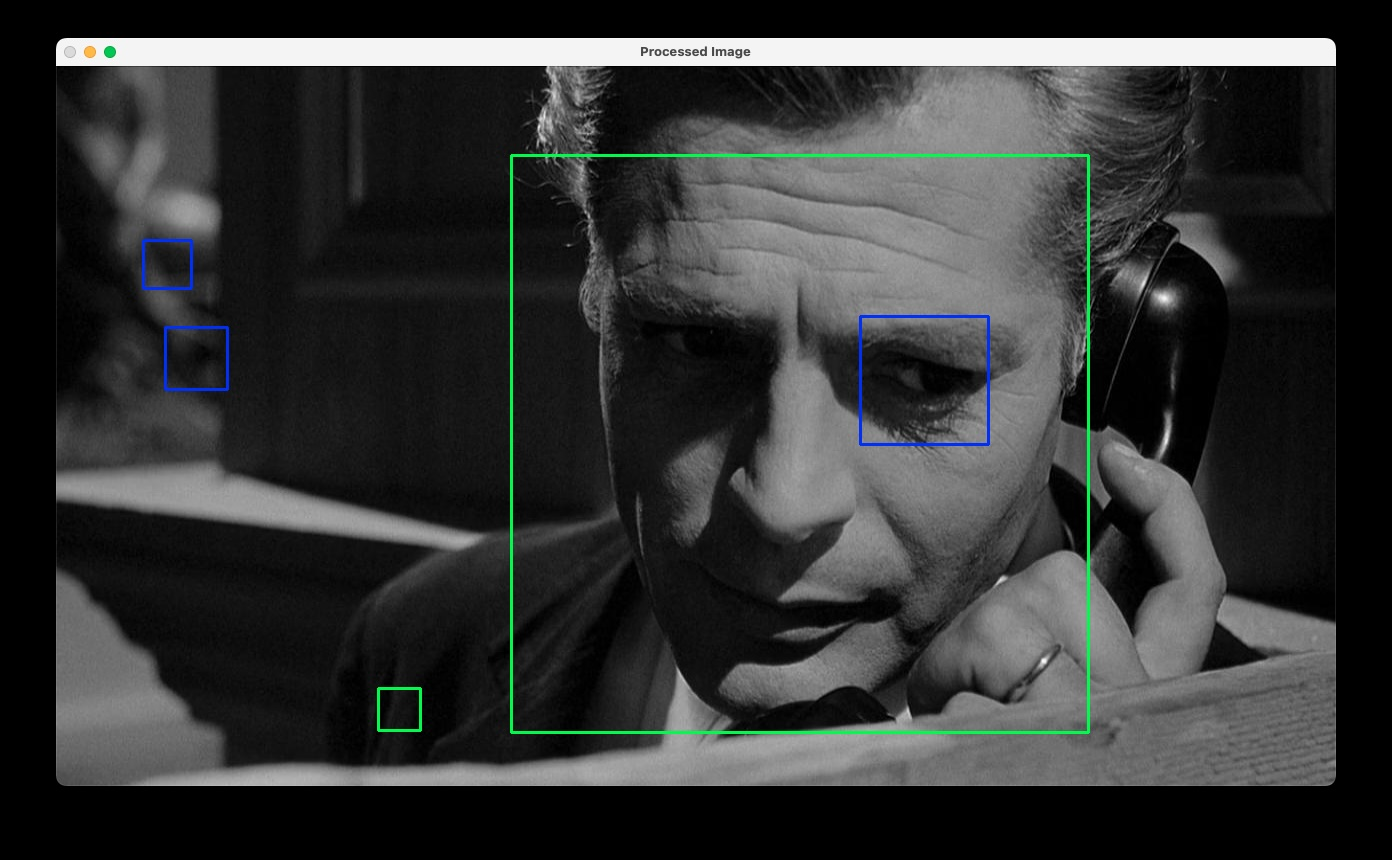
\includegraphics[width=0.32\textwidth]{result_images/closeup/ss9}
            }

            \vspace{1em}

            \subfloat[CLOSE\_UP]{%
                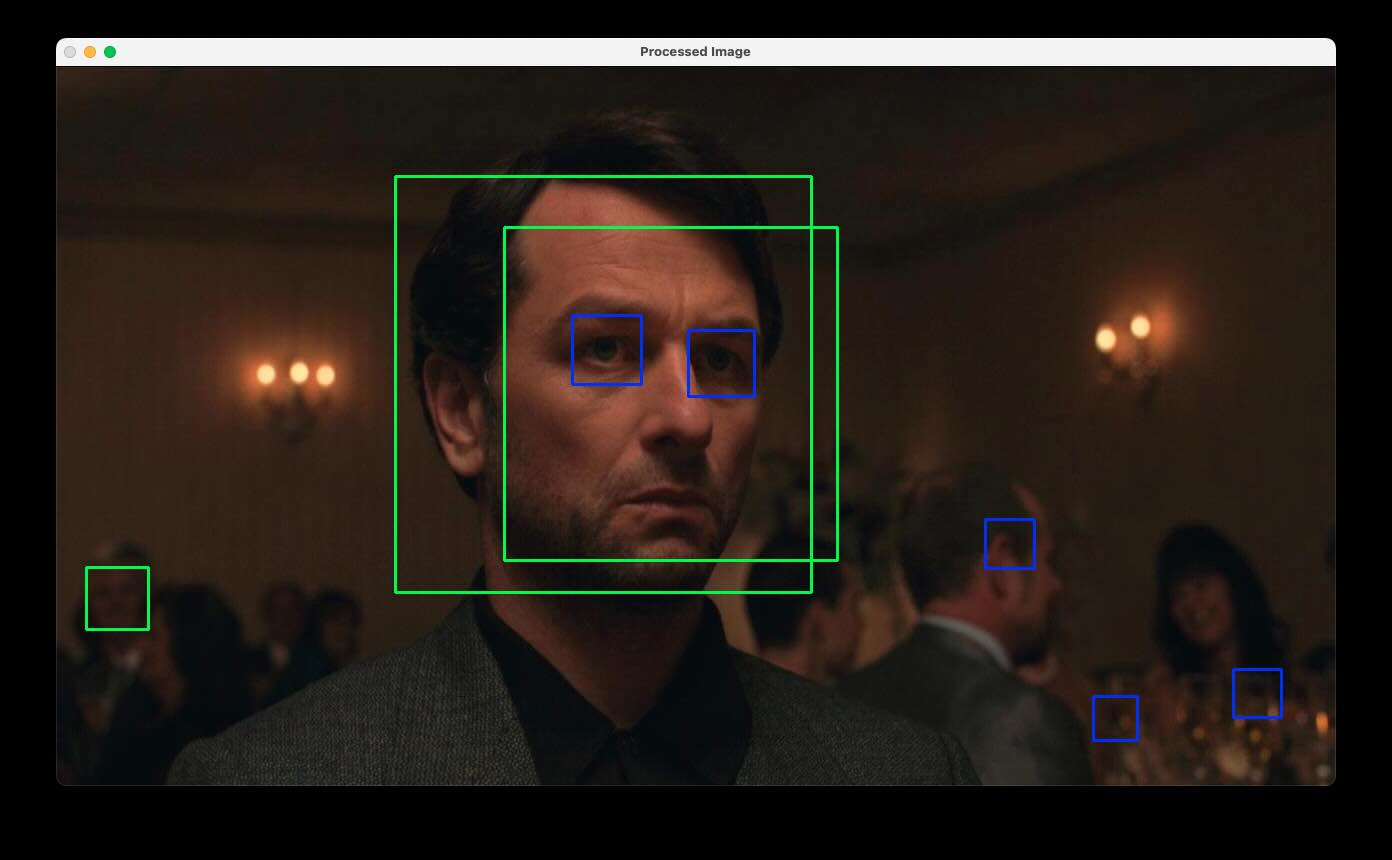
\includegraphics[width=0.32\textwidth]{result_images/closeup/ss10}
            }

            \caption{Examples of close-up shots with classification}
        \end{figure}


		\subsubsection{Medium shots}
		 \begin{figure}[H]
            \centering

            \subfloat[MEDIUM]{%
                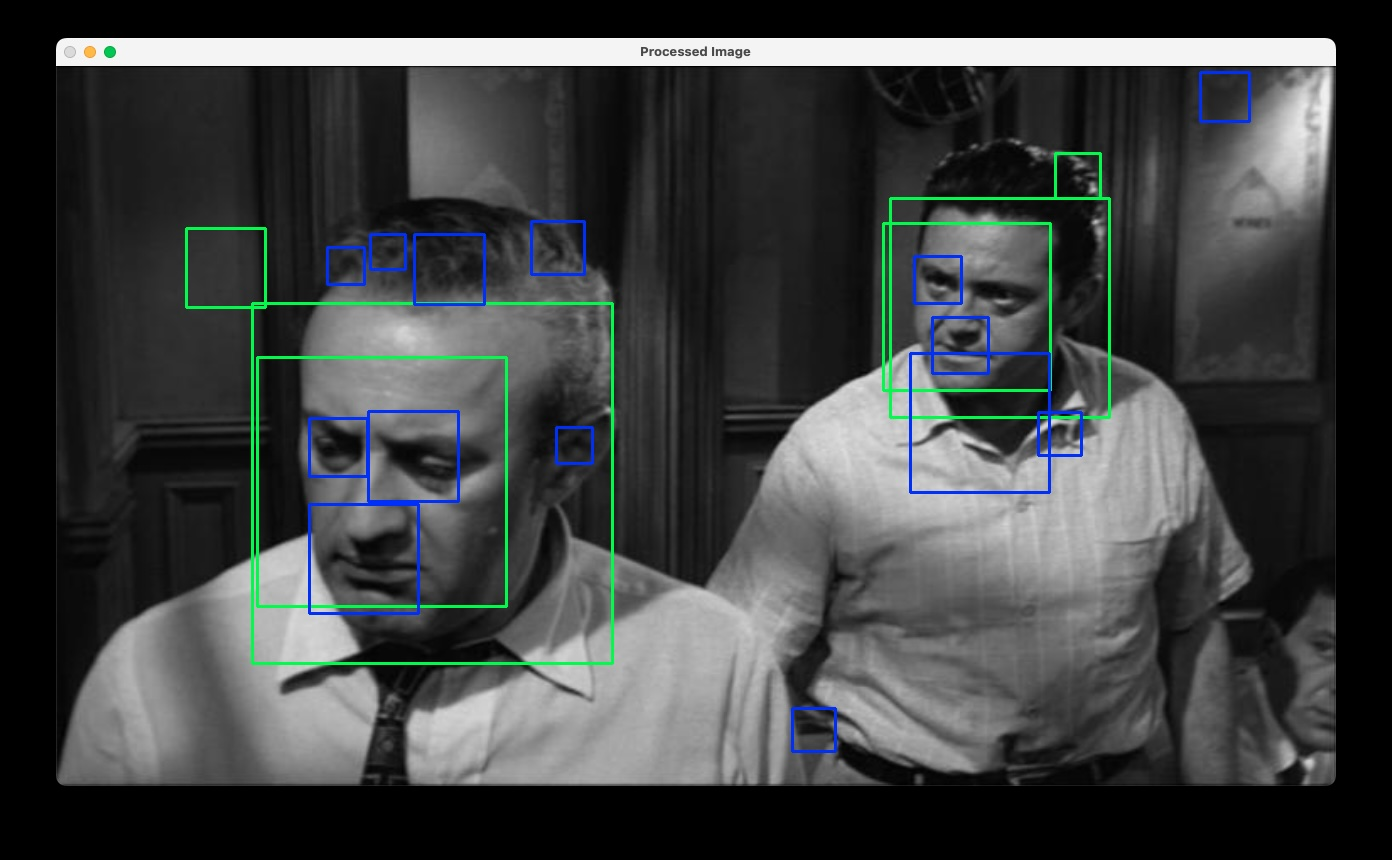
\includegraphics[width=0.32\textwidth]{result_images/medium/ss1}
            }
            \hfill
            \subfloat[MEDIUM]{%
                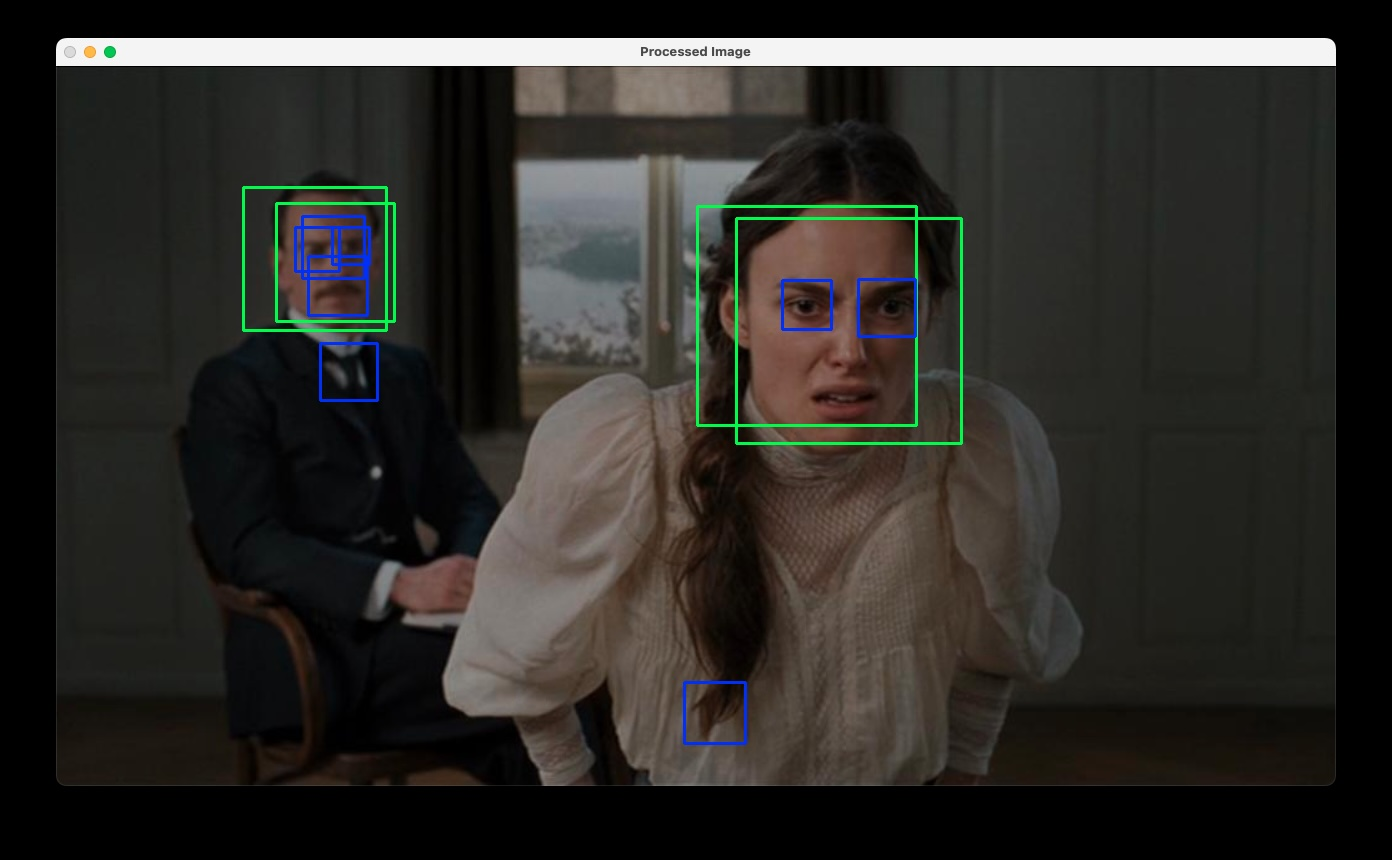
\includegraphics[width=0.32\textwidth]{result_images/medium/ss2}
            }
            \hfill
            \subfloat[MEDIUM]{%
                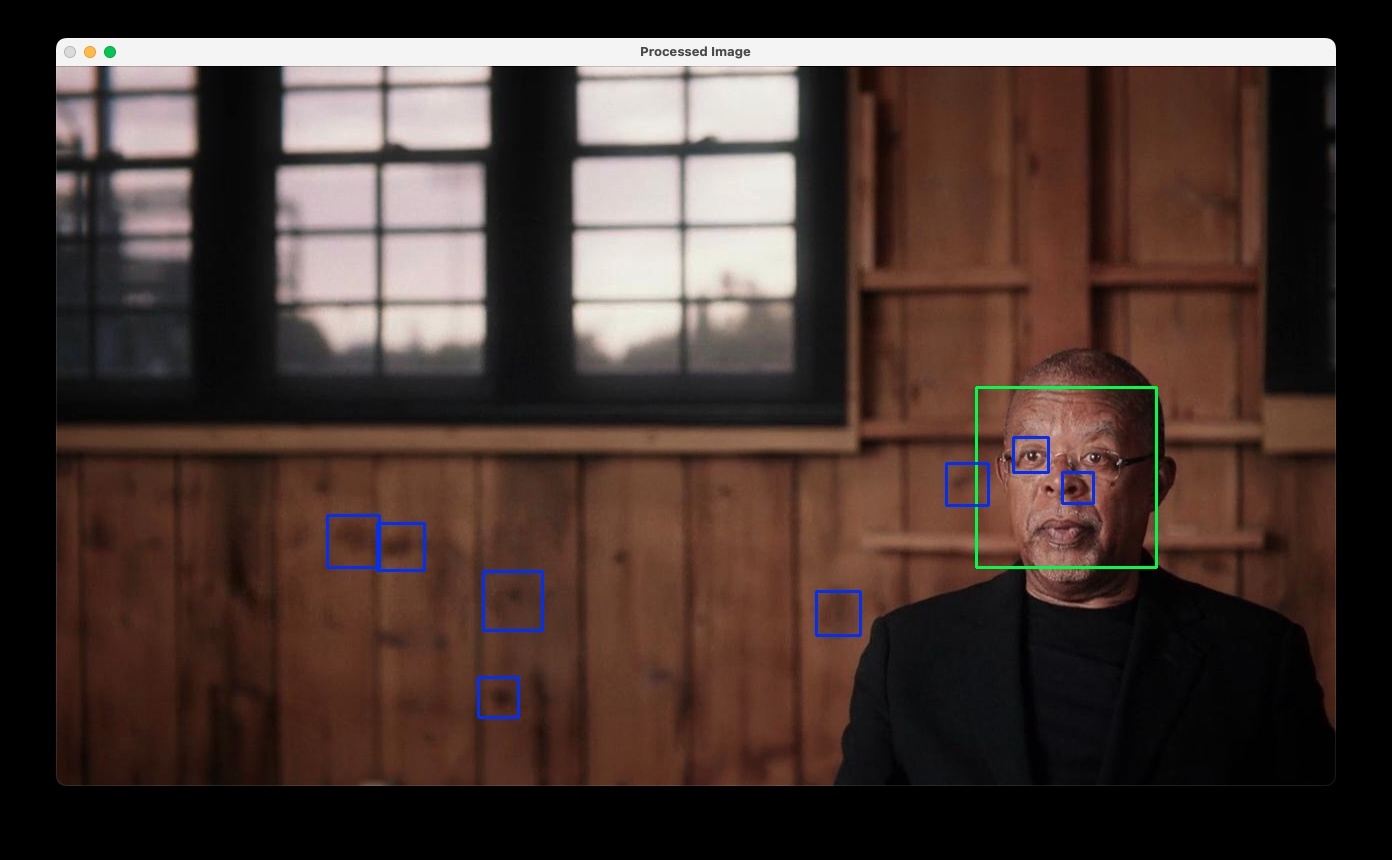
\includegraphics[width=0.32\textwidth]{result_images/medium/ss3}
            }

            \vspace{1em}

            \subfloat[CLOSE\_UP]{%
                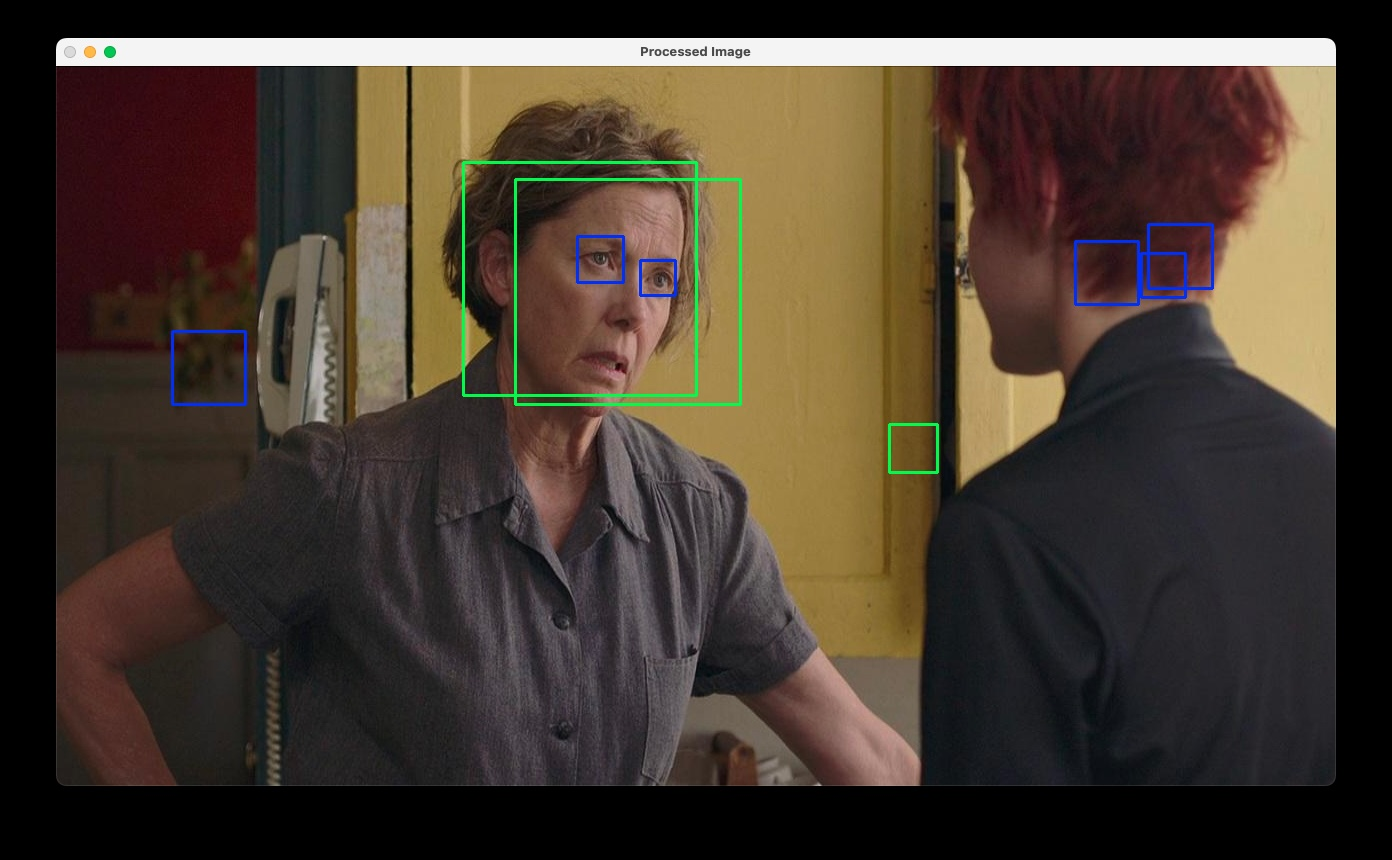
\includegraphics[width=0.32\textwidth]{result_images/medium/ss4}
            }
            \hfill
            \subfloat[MEDIUM]{%
                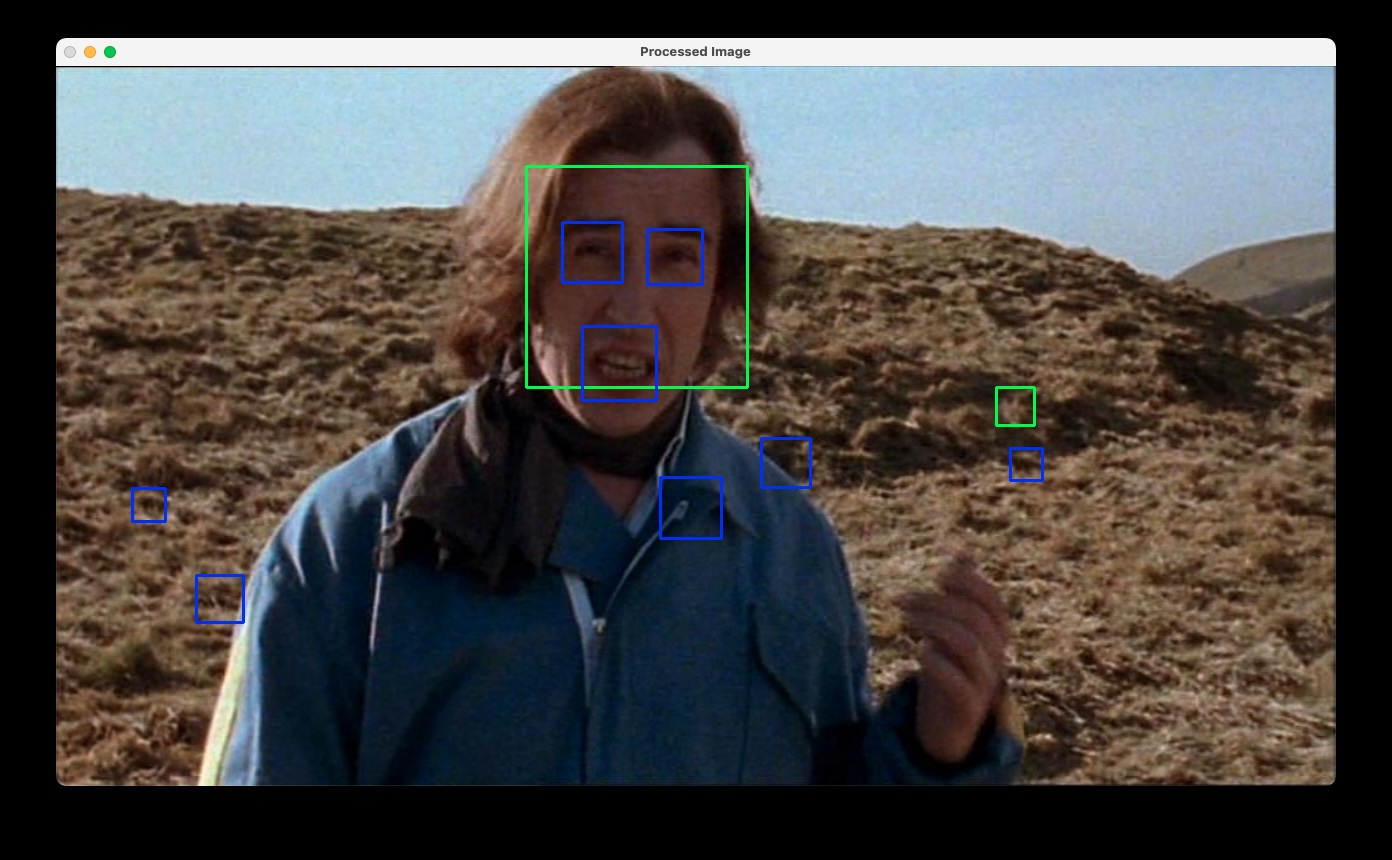
\includegraphics[width=0.32\textwidth]{result_images/medium/ss5}
            }
            \hfill
            \subfloat[MEDIUM]{%
                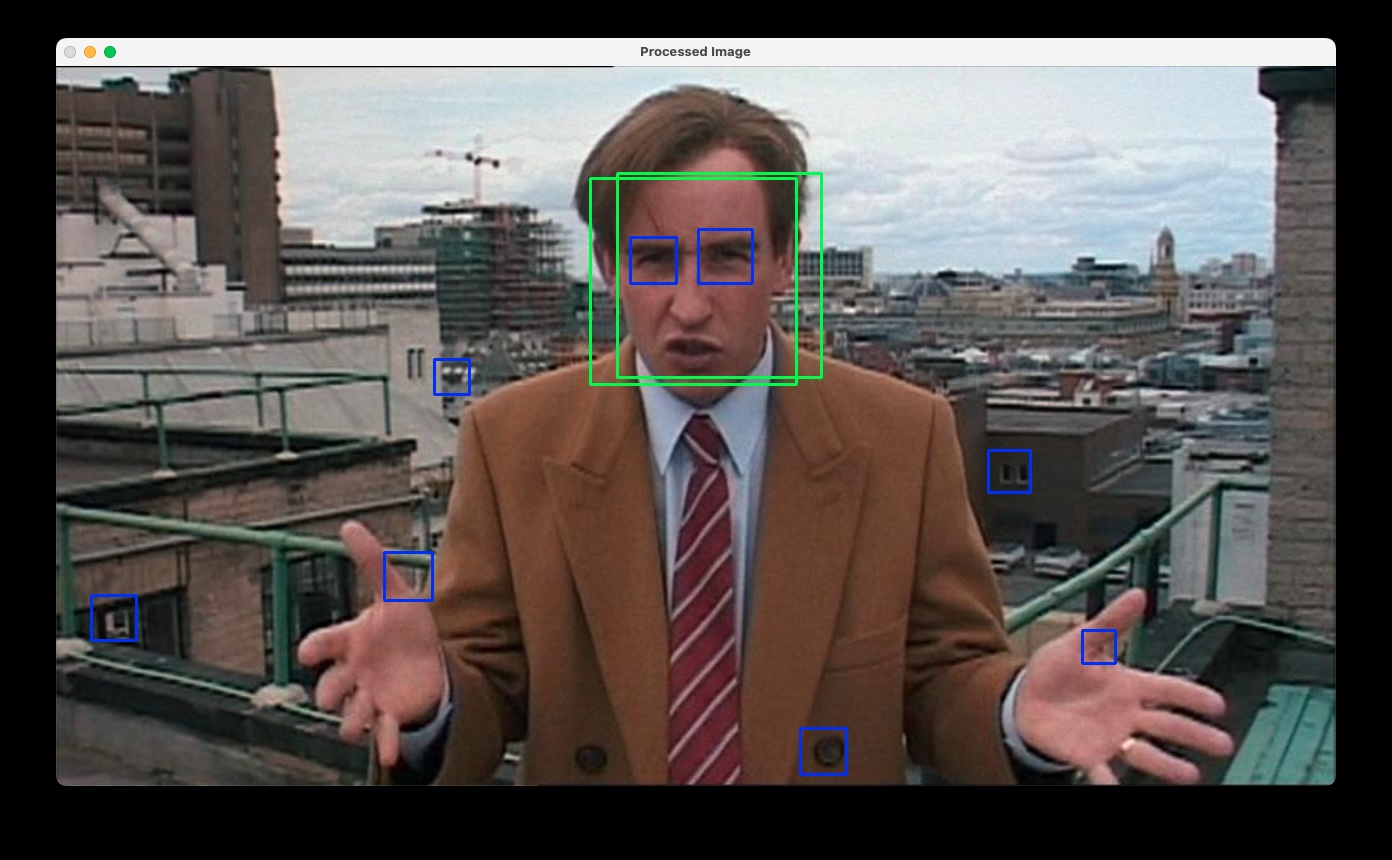
\includegraphics[width=0.32\textwidth]{result_images/medium/ss6}
            }

            \vspace{1em}

            \subfloat[MEDIUM]{%
                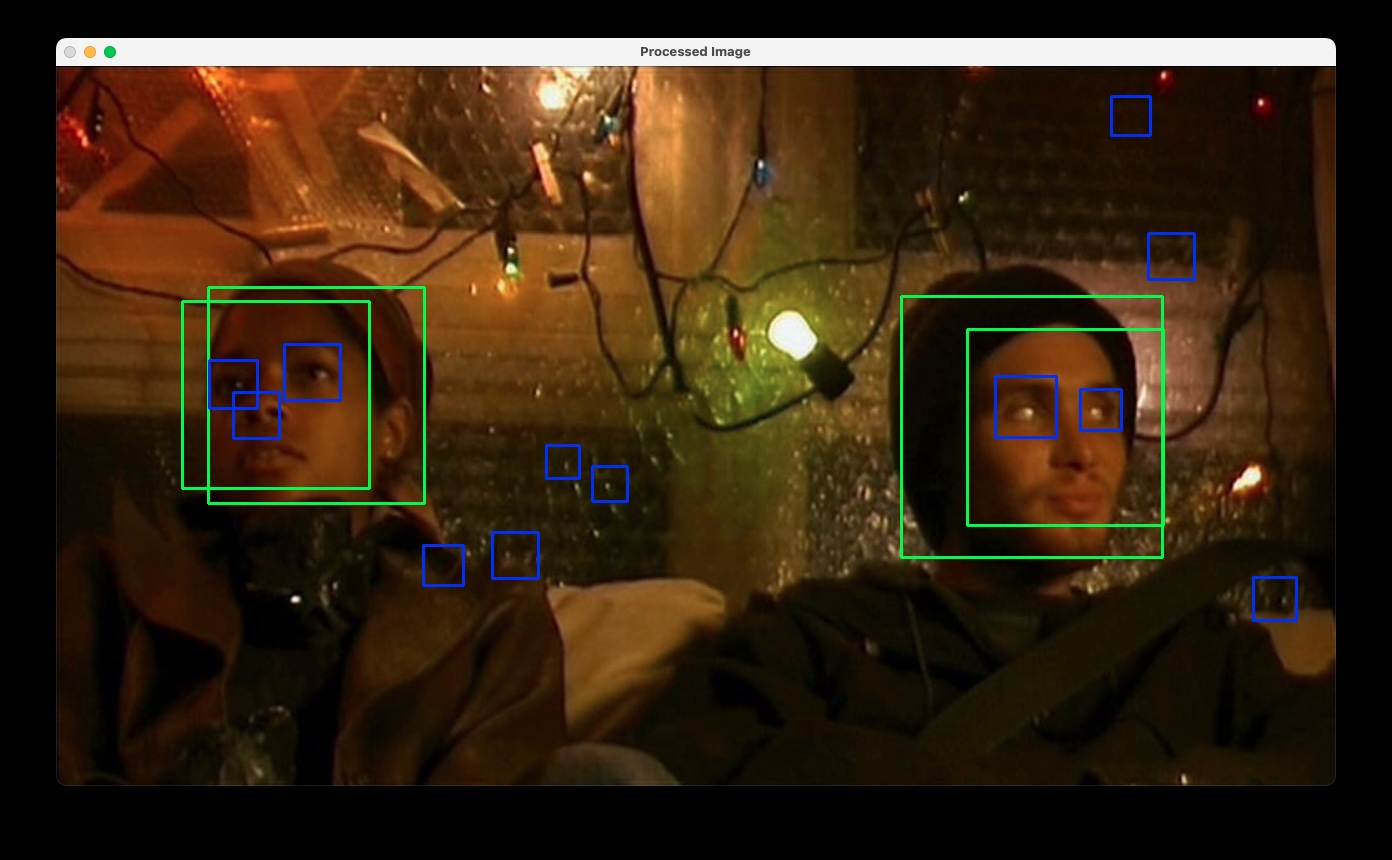
\includegraphics[width=0.32\textwidth]{result_images/medium/ss7}
            }
            \hfill
            \subfloat[MEDIUM]{%
                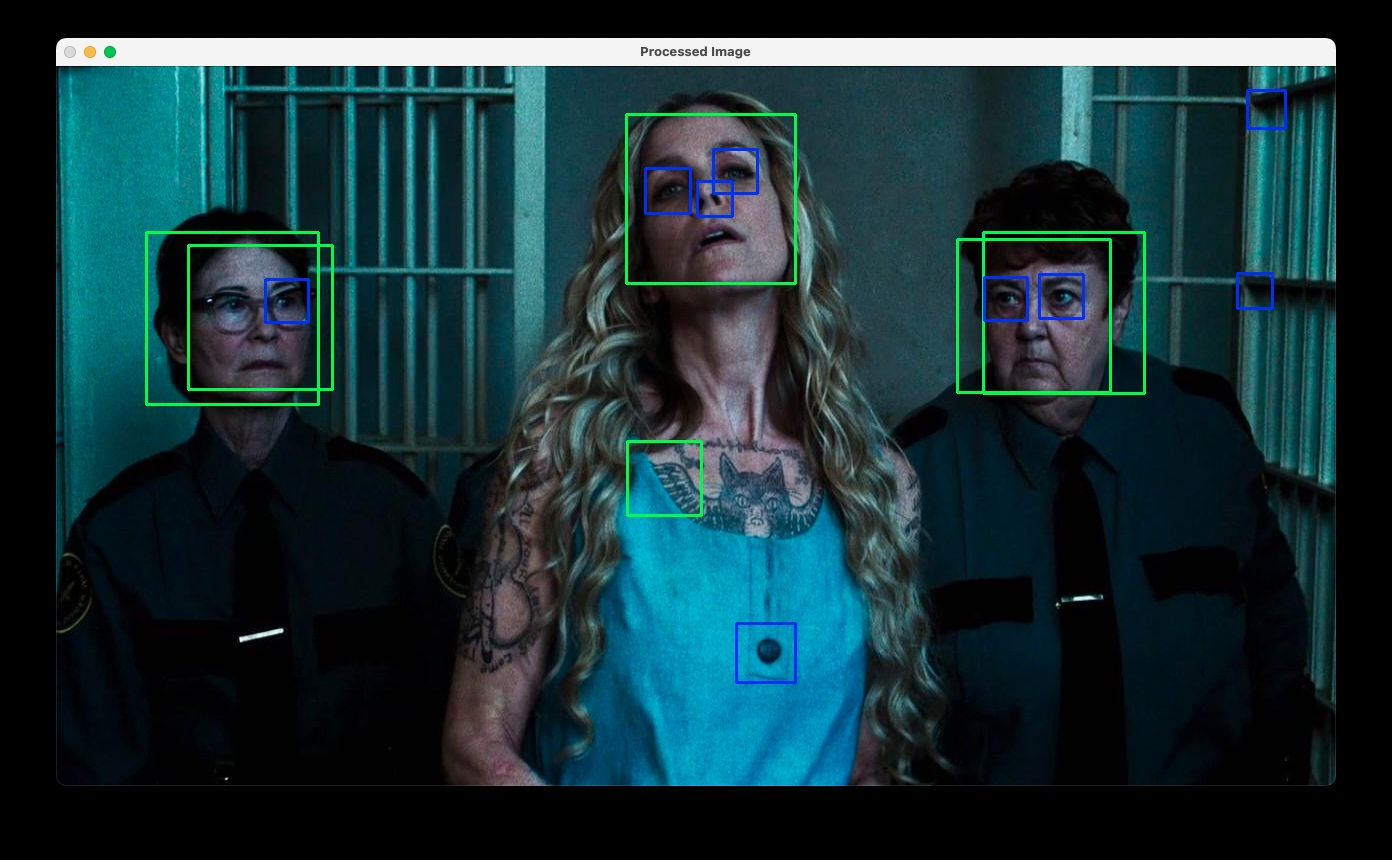
\includegraphics[width=0.32\textwidth]{result_images/medium/ss8}
            }
            \hfill
            \subfloat[WIDE]{%
                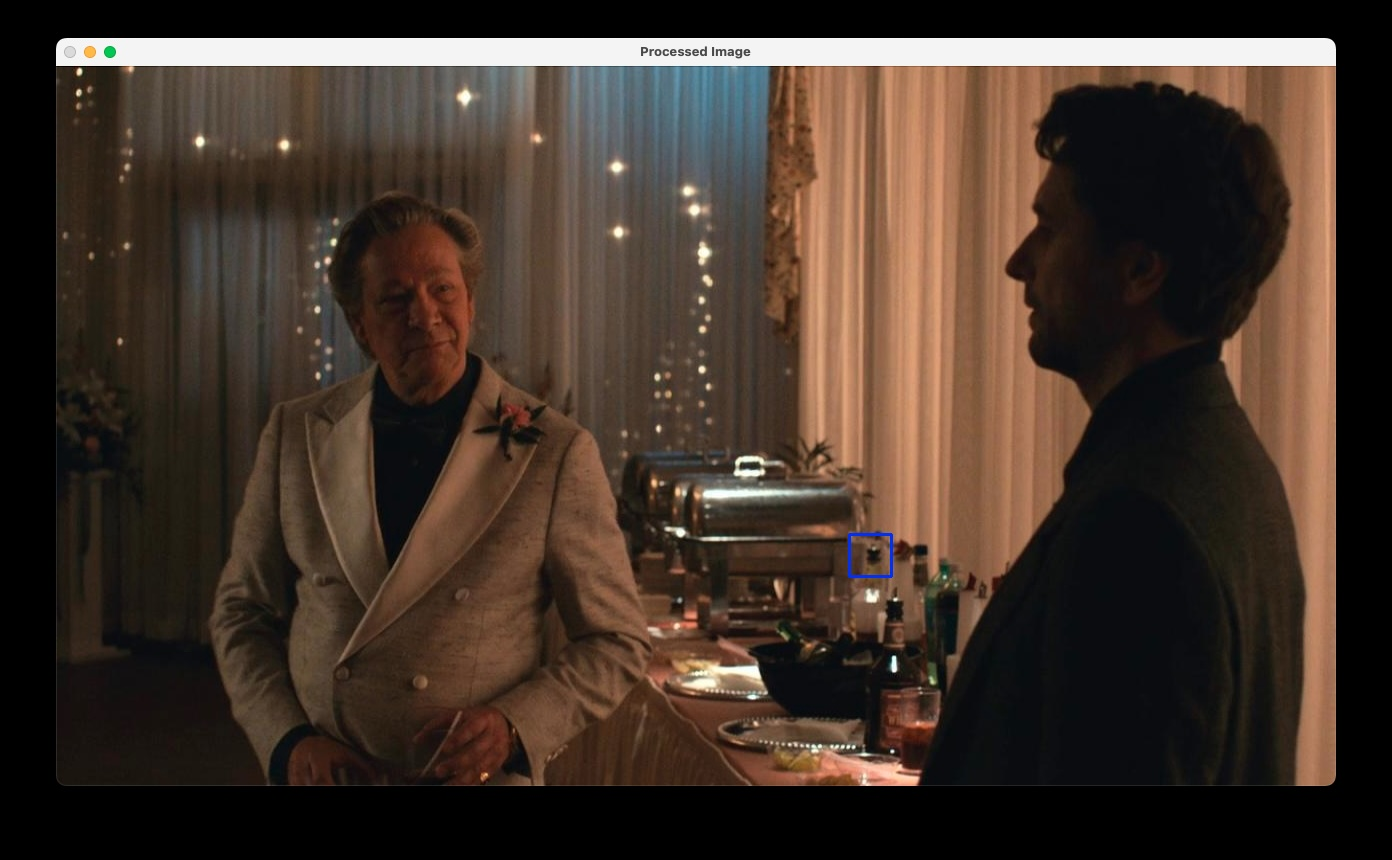
\includegraphics[width=0.32\textwidth]{result_images/medium/ss9}
            }

            \vspace{1em}

            \subfloat[MEDIUM]{%
                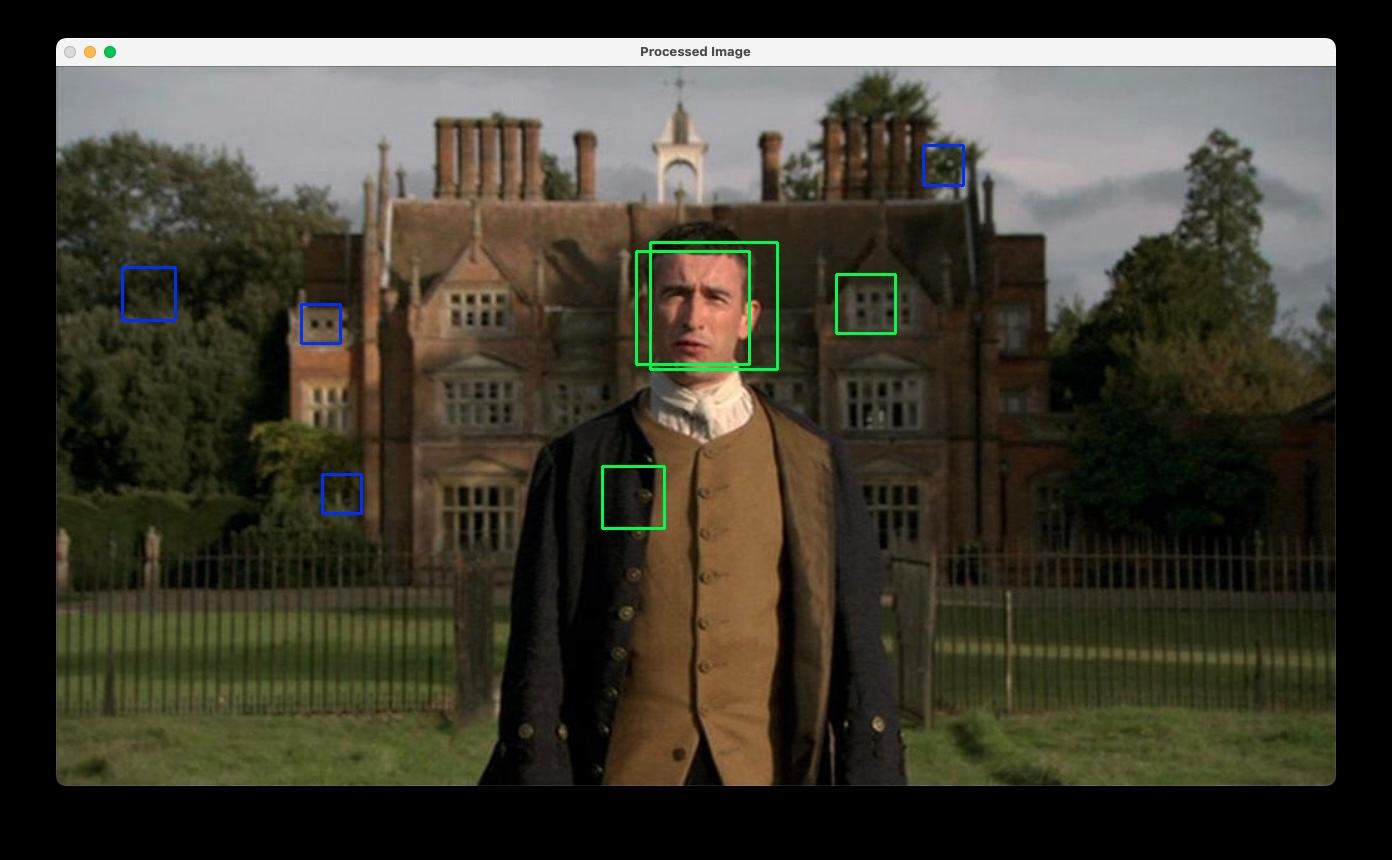
\includegraphics[width=0.32\textwidth]{result_images/medium/ss10}
            }

            \caption{Examples of medium shots with classification}
        \end{figure}

	\subsubsection{Wide shots}
		 \begin{figure}[H]
            \centering

            \subfloat[WIDE]{%
                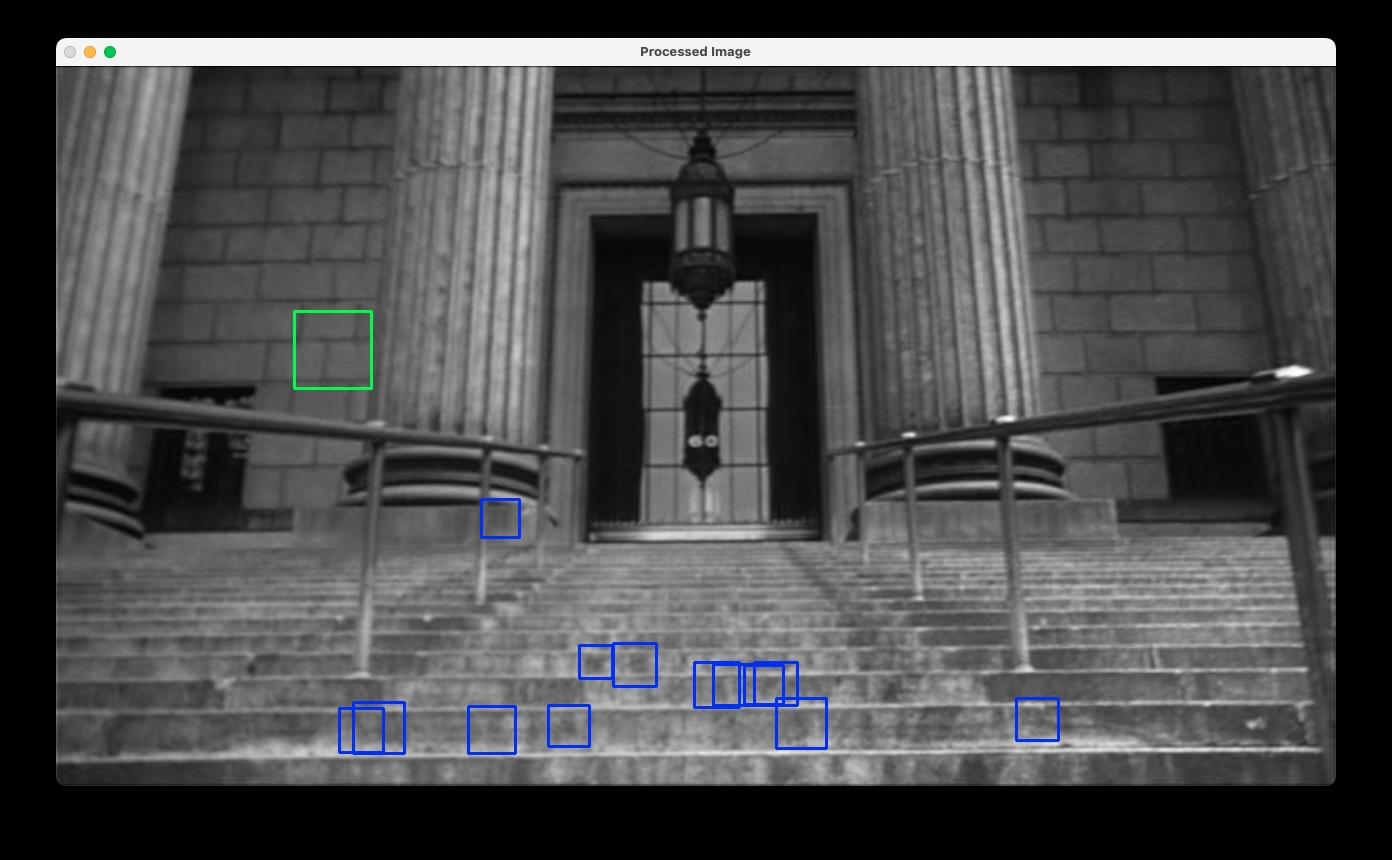
\includegraphics[width=0.32\textwidth]{result_images/wide/ss1}
            }
            \hfill
            \subfloat[WIDE]{%
                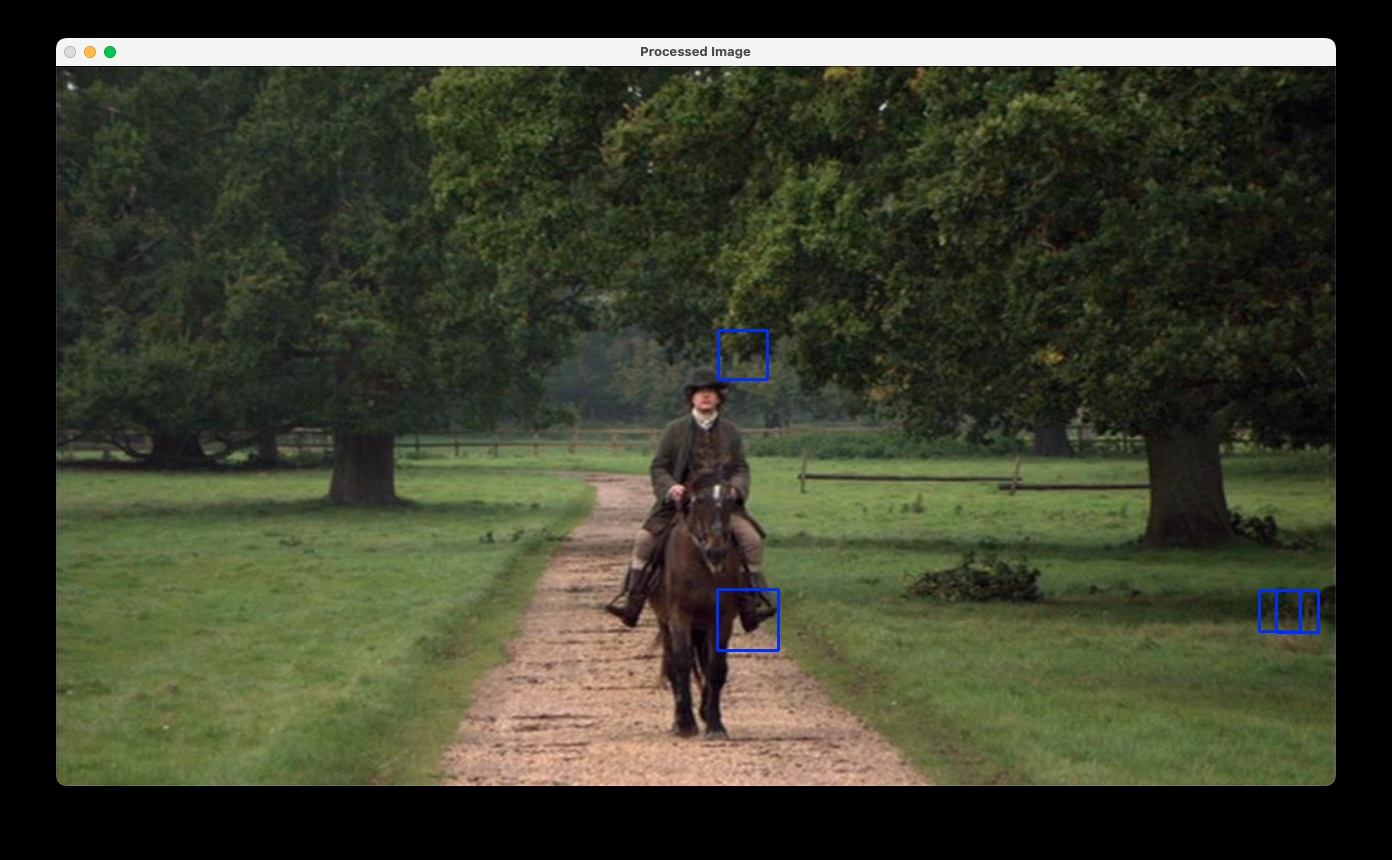
\includegraphics[width=0.32\textwidth]{result_images/wide/ss2}
            }
            \hfill
            \subfloat[WIDE]{%
                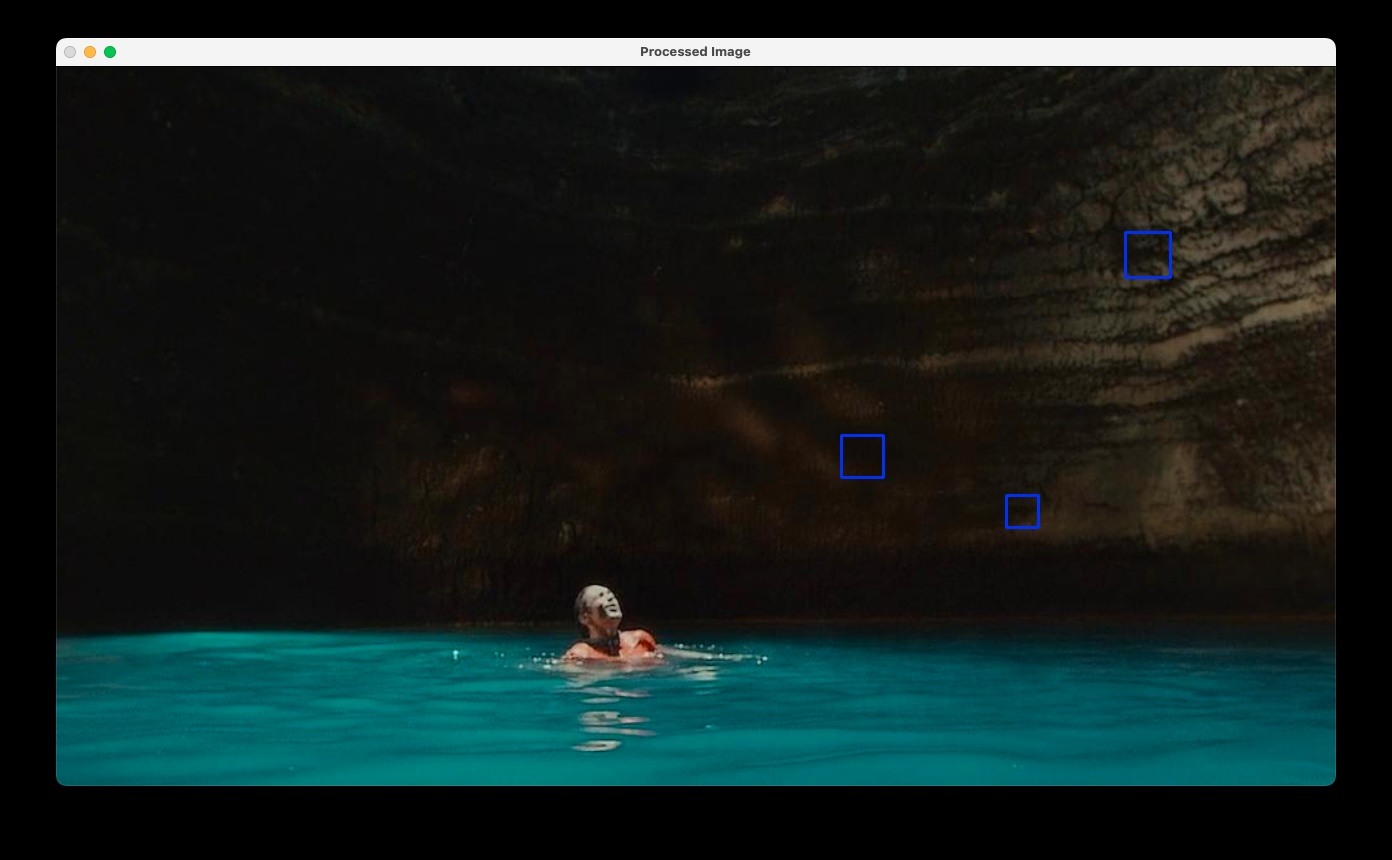
\includegraphics[width=0.32\textwidth]{result_images/wide/ss3}
            }

            \vspace{1em}

            \subfloat[MEDIUM]{%
                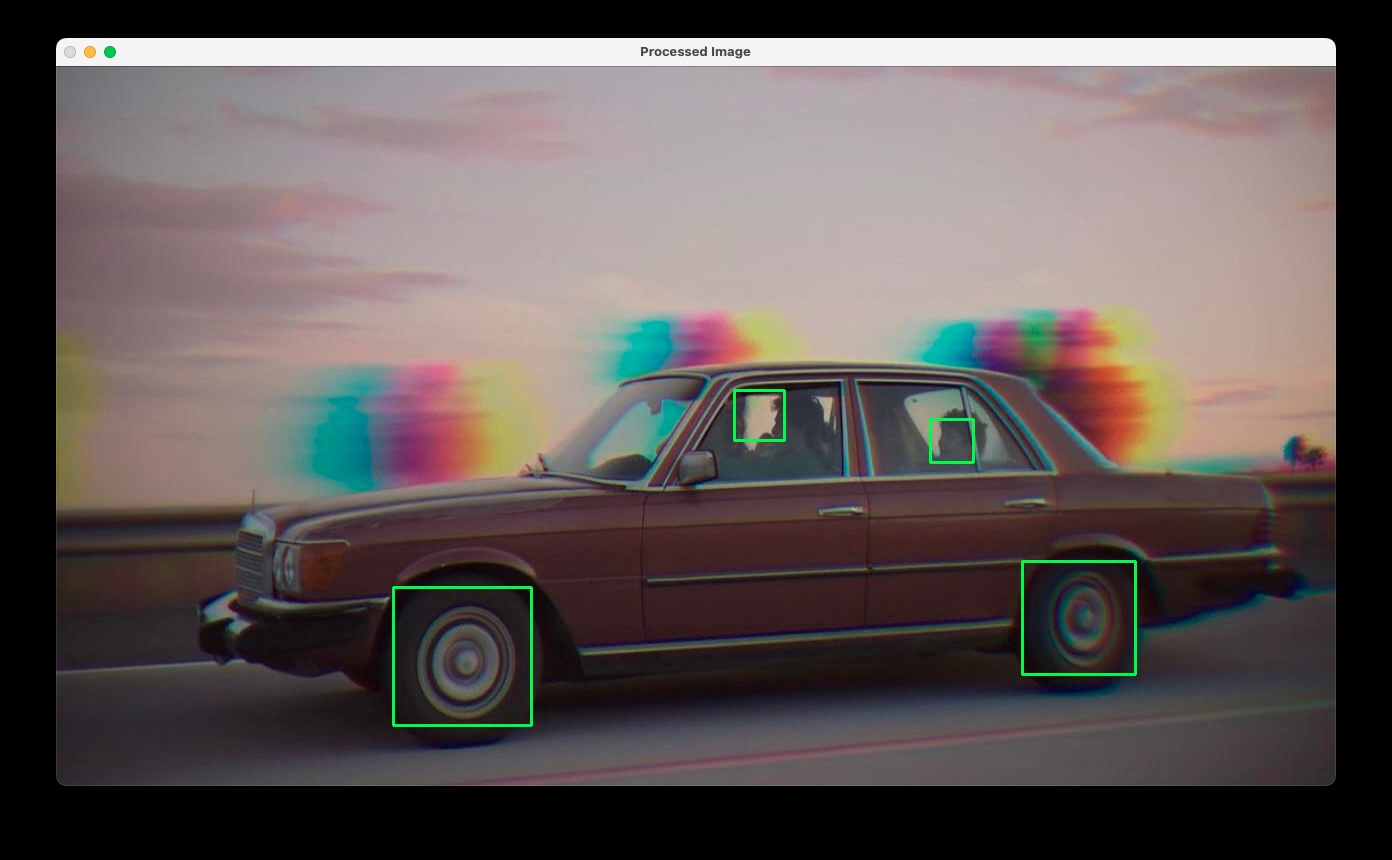
\includegraphics[width=0.32\textwidth]{result_images/wide/ss4}
            }
            \hfill
            \subfloat[WIDE]{%
                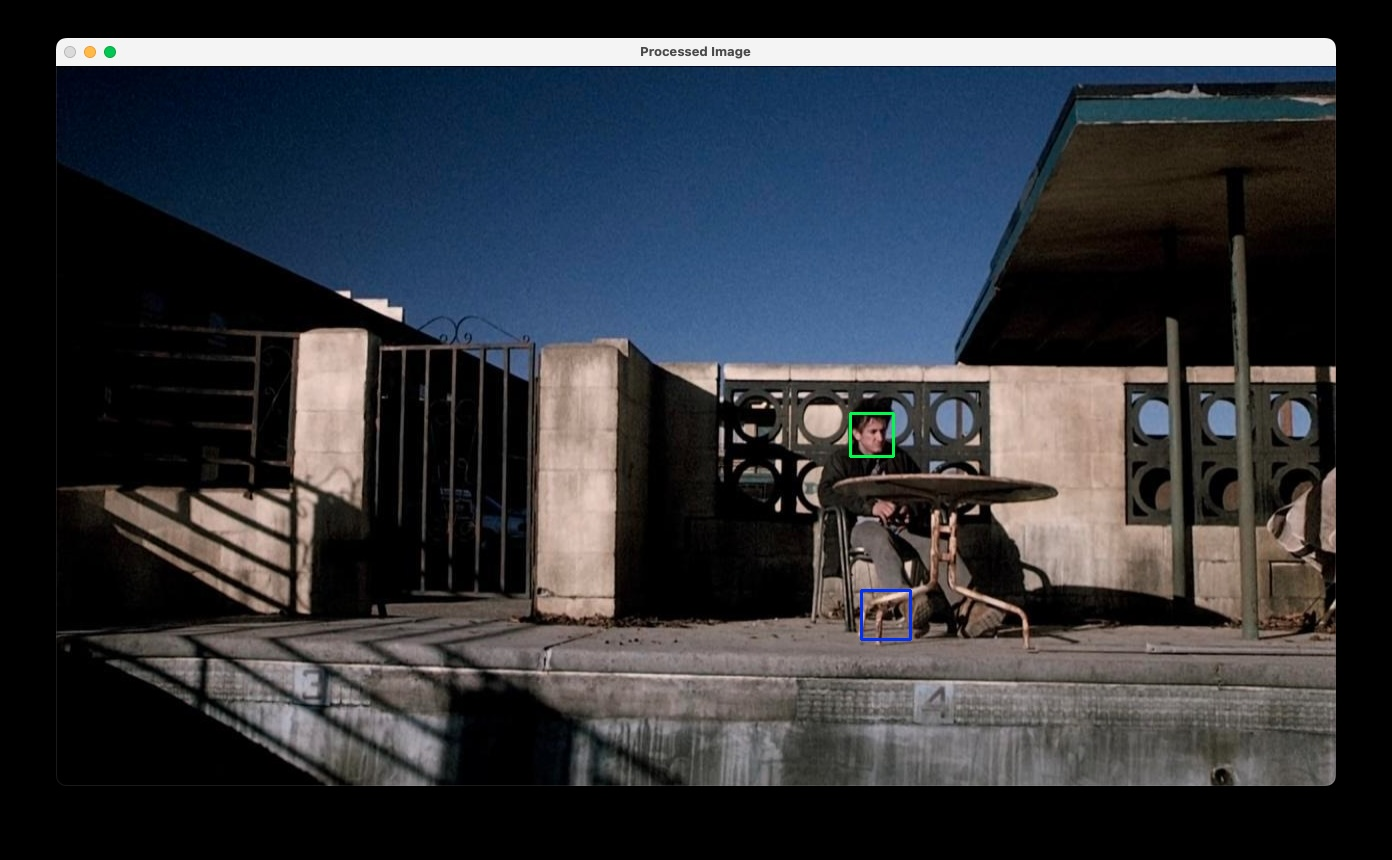
\includegraphics[width=0.32\textwidth]{result_images/wide/ss5}
            }
            \hfill
            \subfloat[WIDE]{%
                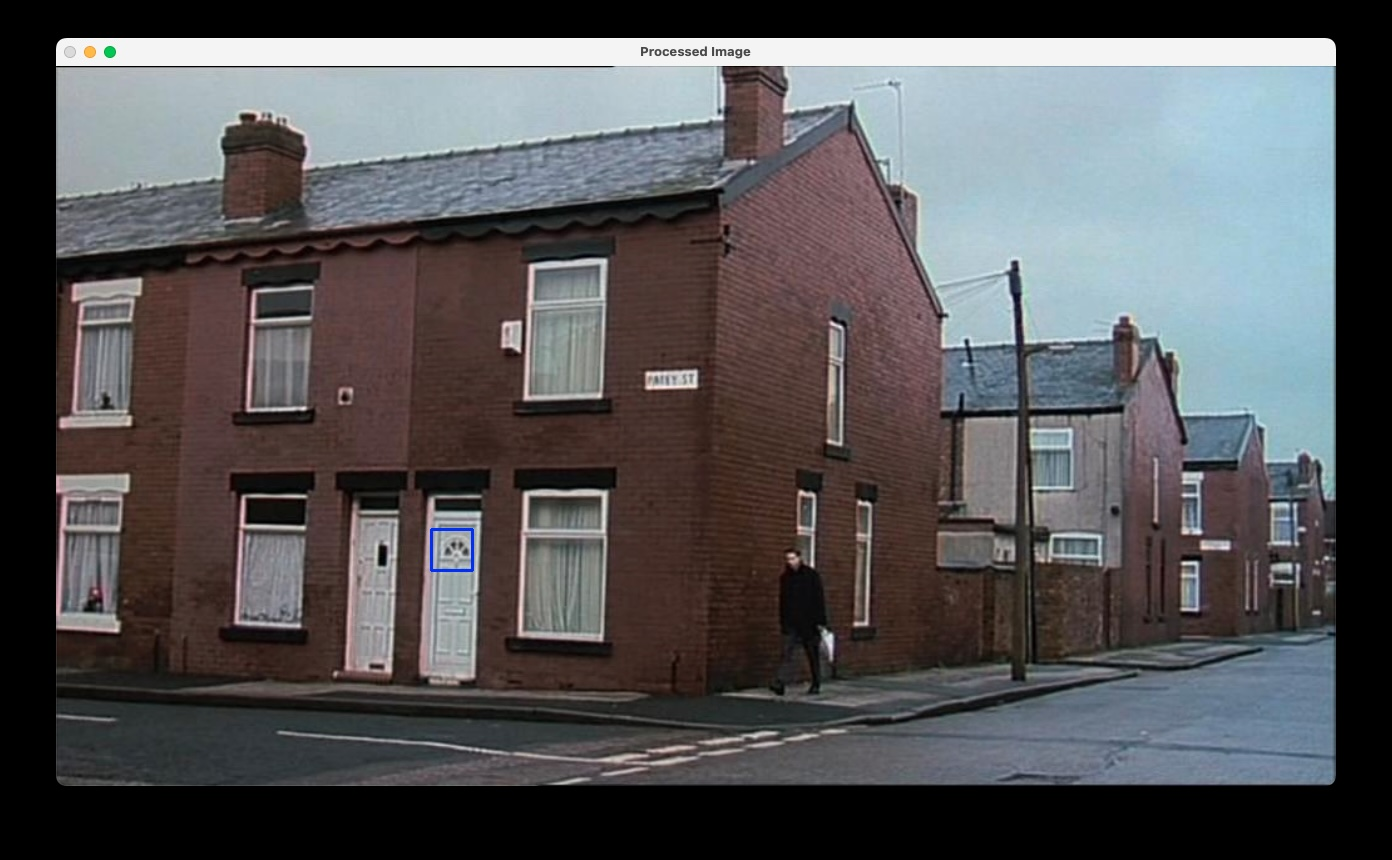
\includegraphics[width=0.32\textwidth]{result_images/wide/ss6}
            }

            \vspace{1em}

            \subfloat[WIDE]{%
                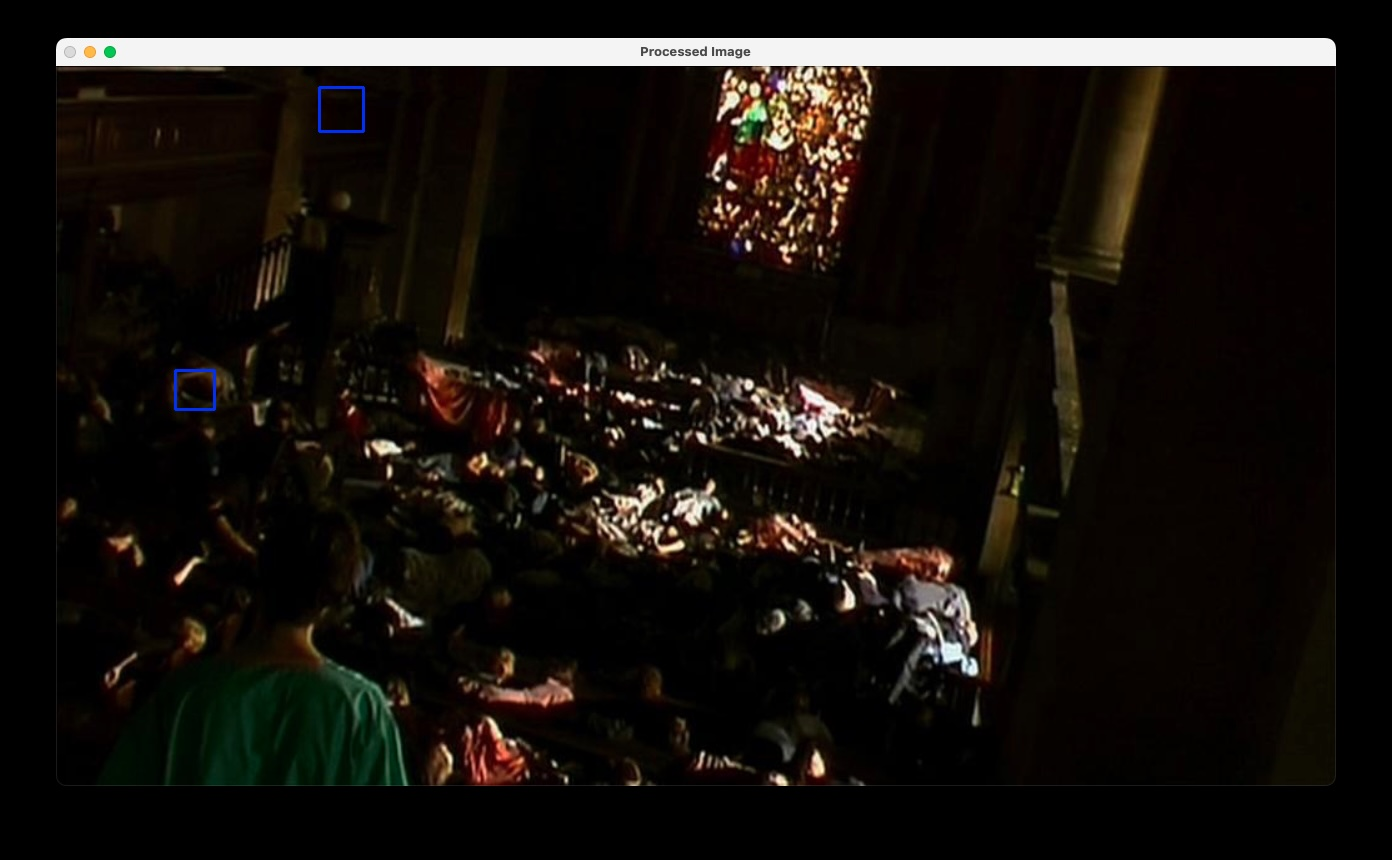
\includegraphics[width=0.32\textwidth]{result_images/wide/ss7}
            }
            \hfill
            \subfloat[WIDE]{%
                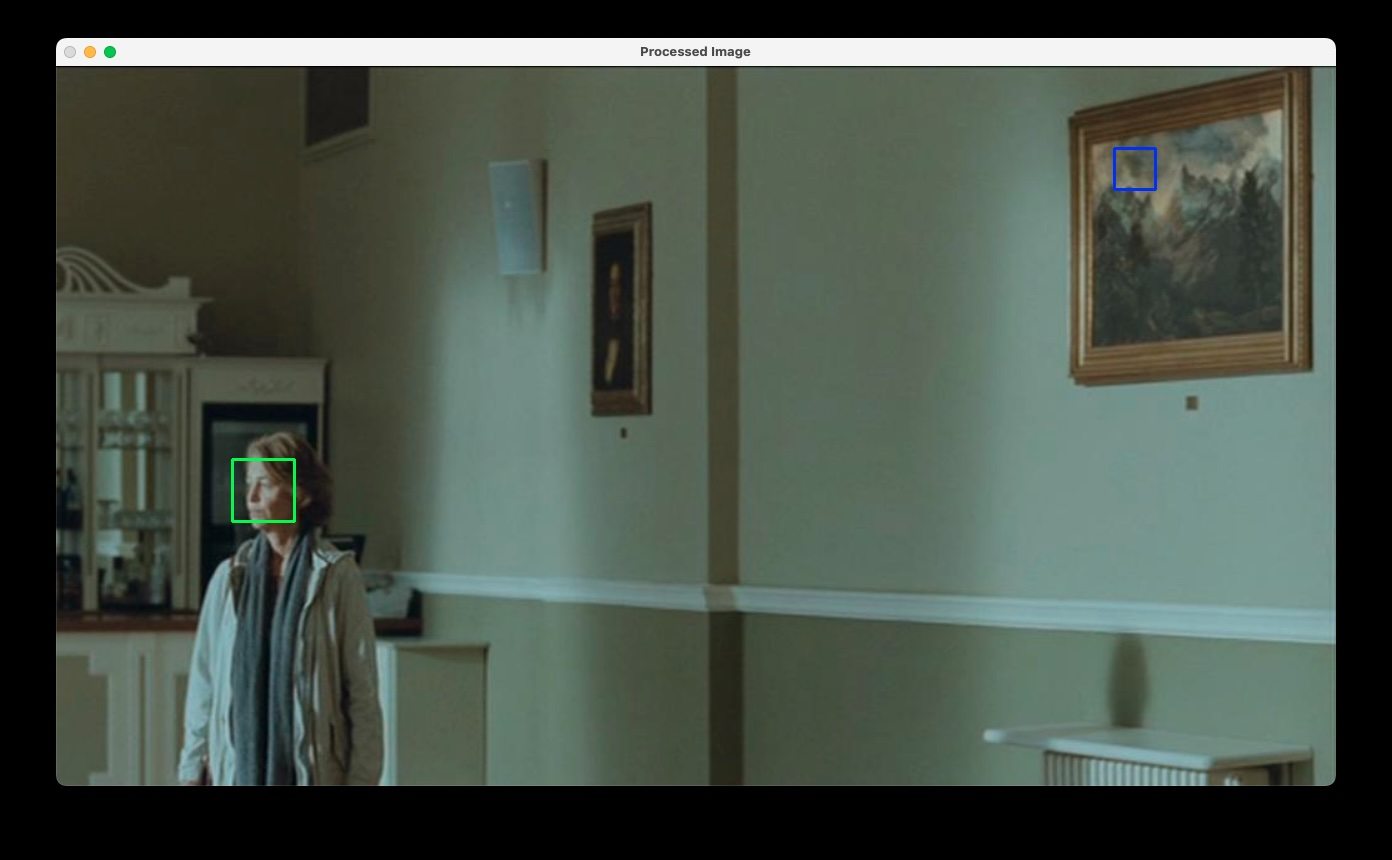
\includegraphics[width=0.32\textwidth]{result_images/wide/ss8}
            }
            \hfill
            \subfloat[WIDE]{%
                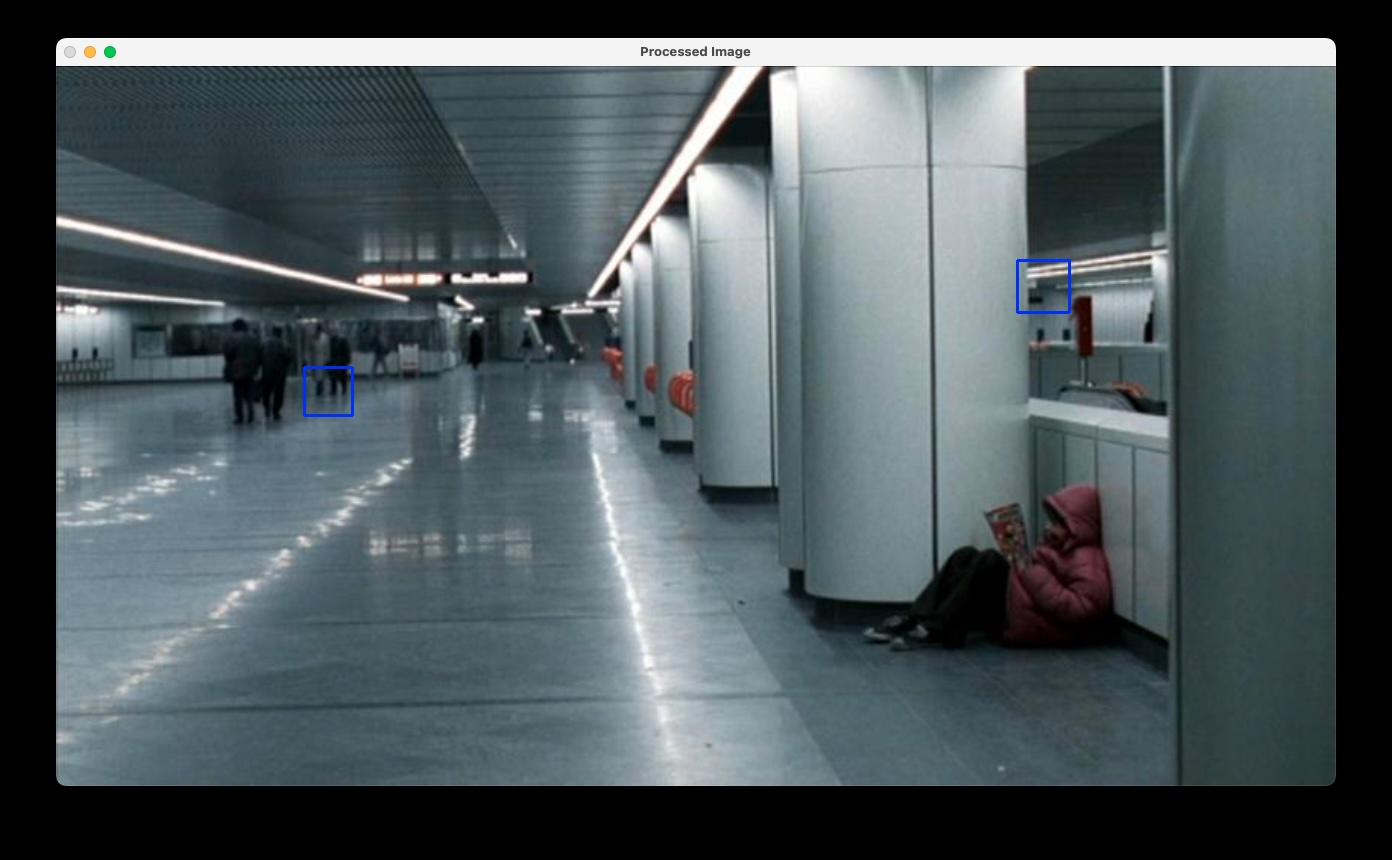
\includegraphics[width=0.32\textwidth]{result_images/wide/ss9}
            }

            \vspace{1em}

            \subfloat[WIDE]{%
                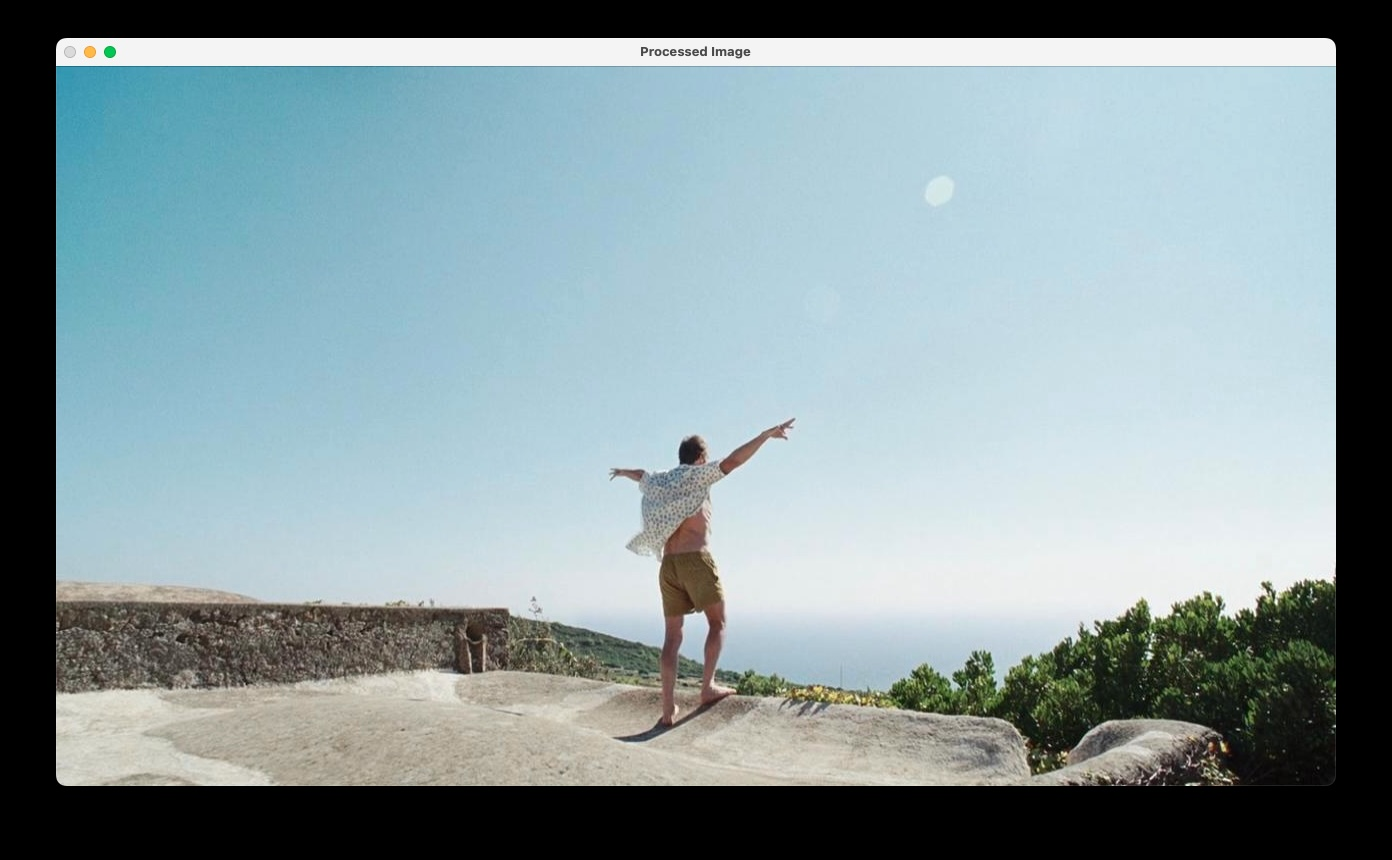
\includegraphics[width=0.32\textwidth]{result_images/wide/ss10}
            }

            \caption{Examples of wide shots with classification}
        \end{figure}


	\subsection{Video Evaluation}
		\paragraph{}
			With video we have more parameters to evaluate such as detection times and we can also
			have a look on some statistics.

		\paragraph{}
			As testing video we used triler for Avengers \cite{marvel}. We choose this type of video, because
			we wanted to get diverse dataset and triler are full of cuts and differents shot types.
			We also aimed fort short video because altrough Viola\&Johnes is effective algorithm, appliing it 
			on the video was computationally expansoive and takes significan amount of time. The sample video duration is 2:24.

		\paragraph{}
			We used time measurements for optimizing our algorithm, but as every machine is unique, we cant provide
			processing time as metric. So processing time is only to imagine how long it to compute.
			For reference tests were ran on Macbook 14 pro 2021 (8 CPU, 14 GPU).

			But we can demonstrate here how well is our optimizer working
		
		\subsubsection{Accuracy}
			\paragraph{}
			We are gonna analyze first 30 seconds of our video. As reference we have manually classified data. It is important to mention
			the setup of algorithm, we can see it at pricture \ref{fig:video_setup}.

			\paragraph{}
			Parameters of optimizer are described at \ref{optimizer}, resolution parameters are for resizing the image and last 3 treshold are tresholds for classification.
			We also use histogram equalization in preprocessing stage.

			\begin{figure}[H]
				\centering
				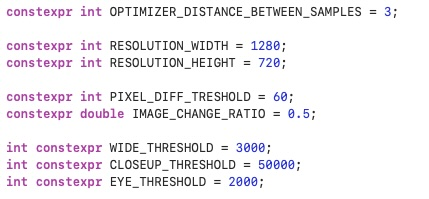
\includegraphics[width=0.5\textwidth]{figures/video setup.jpg}
				\caption{Algorithm setup for video classification}
				\label{fig:video_setup}
			\end{figure}


		
		% \begin{table}[H]
		% 	\centering
		% 	\begin{tabular}{|l|l|lll}
		% 		\cline{1-2}
		% 		Time {[}ms{]} & Shot Type &  &  &  \\ \cline{1-2}
		% 		0             & WIDE      &  &  &  \\ \cline{1-2}
		% 		4840          & CLOSE     &  &  &  \\ \cline{1-2}
		% 		7760          & WIDE      &  &  &  \\ \cline{1-2}
		% 		8800          & MEDIUM    &  &  &  \\ \cline{1-2}
		% 		10000         & MEDIUM    &  &  &  \\ \cline{1-2}
		% 		12700         & WIDE      &  &  &  \\ \cline{1-2}
		% 		15300         & CLOSE     &  &  &  \\ \cline{1-2}
		% 		17000         & CLOSE     &  &  &  \\ \cline{1-2}
		% 		19000         & WIDE      &  &  &  \\ \cline{1-2}
		% 		25300         & MEDUIM    &  &  &  \\ \cline{1-2}
		% 		26900         & CLOSE     &  &  &  \\ \cline{1-2}
		% 		28500         & WIDE      &  &  &  \\ \cline{1-2}
		% 	\end{tabular}
		% 	\caption{Manual classification of first 30s of sample video}
		% \end{table}

		\begin{figure}[H]
			\centering
			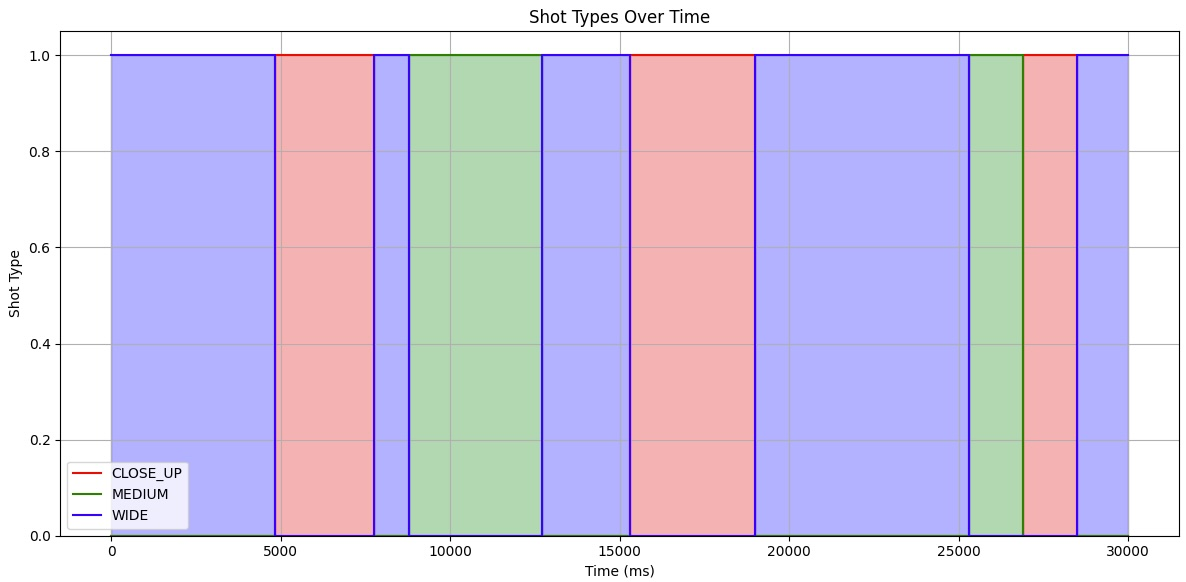
\includegraphics[width=0.8\textwidth]{figures/marvel_ref_graph.jpg}
			\caption{Manually classified video \cite{marvel}}
			\label{fig:marvel_ref}
		\end{figure}

		\begin{figure}[H]
			\centering
			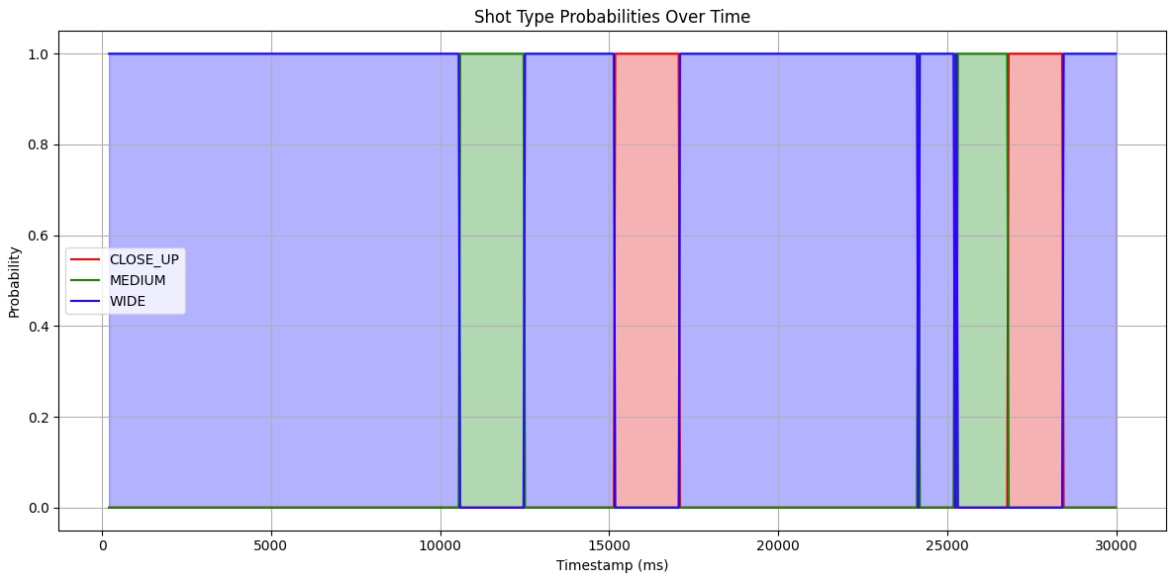
\includegraphics[width=0.8\textwidth]{figures/marvel_real_graph.jpg}
			\caption{Classification with Viola\&Johnes}
			\label{fig:marvel_real}
		\end{figure}

		Notice that Viola\&Johnes classification has small delay, described in \ref{filmstats}.

		\begin{table}[H]
			\centering
			\begin{tabular}{|l|l|l|l|}
				\hline
				\textbf{actual/predicted} & \textbf{close} & \textbf{medium} & \textbf{wide} \\ \hline
				\textbf{close}            & 1841,4         & 40,5            & 1858,6        \\ \hline
				\textbf{medium}           & 0,0            & 3624,5          & 25,5          \\ \hline
				\textbf{wide}             & 2997,2         & 1835,0          & 17777,3       \\ \hline
			\end{tabular}
			\caption{Confusion matrix of first 30s of video \cite{marvel}}
			\label{fig:marvel_confusion}
		\end{table}


		\begin{table}[H]
			\centering
			\begin{tabular}{|l|l|l|l|}
				\hline
				\textbf{}            & \textbf{close} & \textbf{medium} & \textbf{wide} \\ \hline
				\textbf{Precision}   & 0,3806         & 0,6590          & 0,9042        \\ \hline
				\textbf{Recall}      & 0,4923         & 0,9930          & 0,7863        \\ \hline
				\textbf{Accuracy}    & 0,8260         & 0,9244          & 0,7758        \\ \hline
				\textbf{F1 score}    & 0,4293         & 0,7922          & 0,8411        \\ \hline
				\textbf{Specificity} & 0,8772         & 0,9127          & 0,7437        \\ \hline
			\end{tabular}
			\caption{Scores of classification of first 30s of video \cite{marvel}}
			\label{fig:marvel_stats}
		\end{table}

	\subsubsection{Optimizer}
		\paragraph{}
			Optimizer significantly improves the performance of the algorithm as we can see in table \ref{marvel_opt}. It 
			also makes classification more stable. See the difference betwen figure \ref{fig:marvel_raw} ad \ref{fig:marvel_real}
		\begin{table}[H]
			\centering
			\begin{tabular}{|l|l|l|l|l|}
				\hline
				\textbf{}                  & \textbf{Processed} & \textbf{Total} & \textbf{Ratio} & \textbf{Runtime [s]} \\ \hline
				\textbf{with optimizer}    & 235                & 3455           & 0,0680174      & 49,6446          \\ \hline
				\textbf{without optimizer} & 3455               & 3455           & 1              & 601,69           \\ \hline
			\end{tabular}
			\caption{Optimizer performance}
			\label{marvel_opt}
		\end{table}

			\begin{figure}[H]
				\centering
				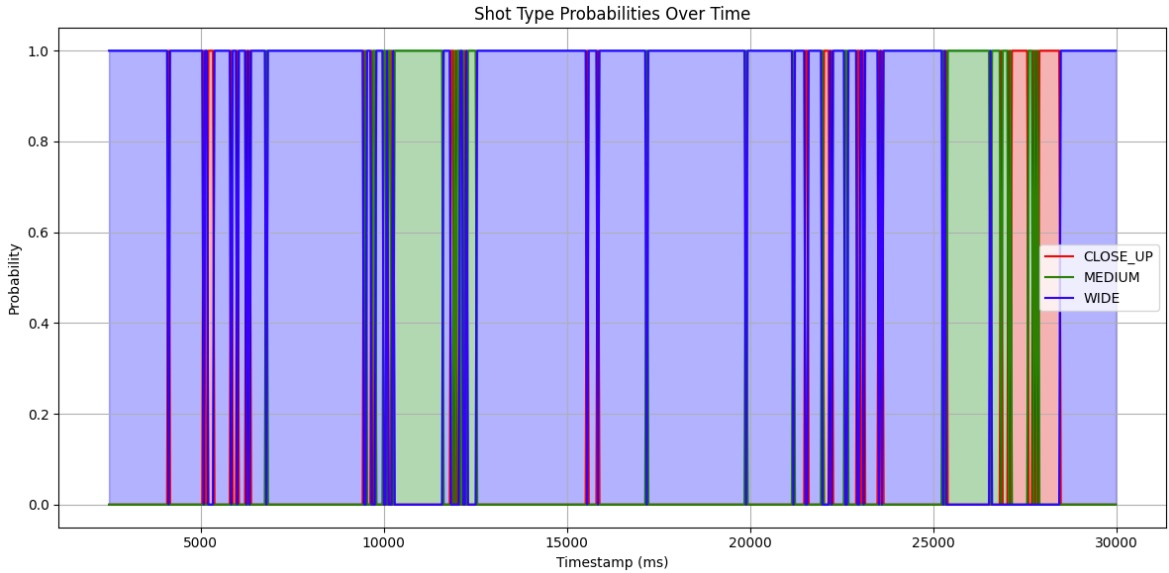
\includegraphics[width=0.8\textwidth]{figures/marvel_raw_graph.jpg}
				\caption{Classification with Viola\&Johnes without the optimizer}
				\label{fig:marvel_raw}
			\end{figure}

		\paragraph{}
			We adding graph, with oversampling turned on to demonstrate function of this feature and also
			make data without optimizer more readable.

			\begin{figure}[H]
				\centering
				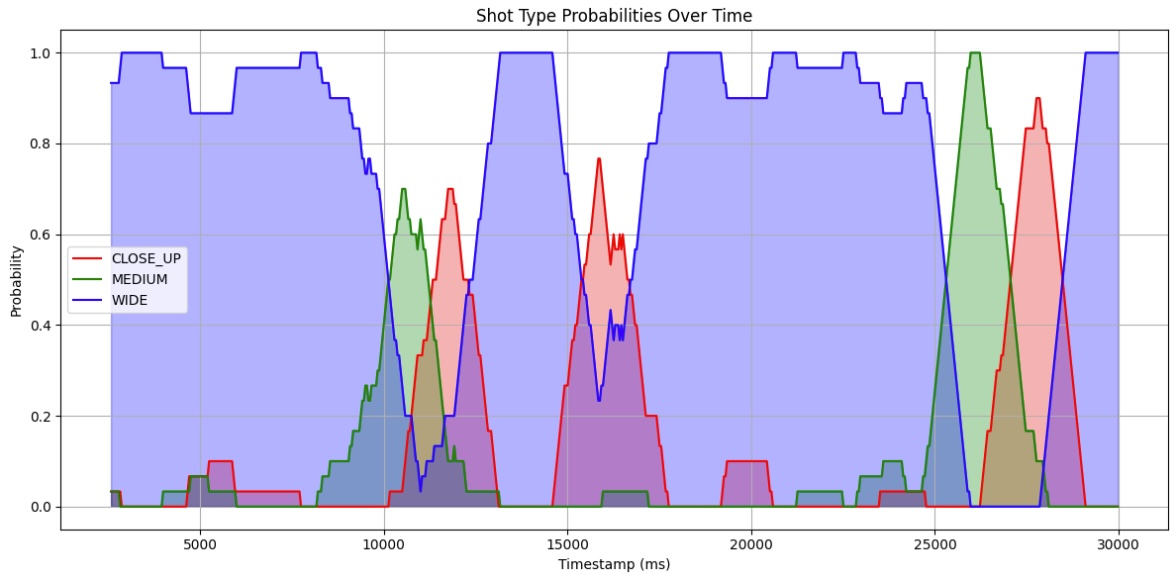
\includegraphics[width=0.8\textwidth]{figures/marvel_oversampled_graph.jpg}
				\caption{Classification with Viola\&Johnes without the optimizer and with oversampling}
				\label{fig:marvel_raw}
			\end{figure}

	





\section{Dataset description}
Miroslaw

\section{Results summary}
Miroslaw
\section{Individual contributions}
both
\section{Conclusion}
Marek


\begin{thebibliography}{1}
	
% 	\bibitem{sx1509}
% 	SX1507/SX1508/SX1509. 2025. \textit{Sparkfun} [online]. [accessed 2025-4-22]. Available at: https://cdn.sparkfun.com/datasheets/BreakoutBoards/sx1509.pdf
	
% 	\bibitem{line_sensor}
% 	Pololu line sensor. 2025. \textit{Pololu.com} [online]. [accessed 2025-4-22]. Available at: https://www.pololu.com/docs/pdf/0J12/QTR-8x.pdf

\end{thebibliography}



% \section{Project overview}
% 	\paragraph{}
% 		The objective of this project was to develop an algorithm capable of detecting objects within a scene.
% The provided data included a training set consisting of images of the target objects, binary masks for separating the objects from the background, and a set of test scenes.
% The expected output of the algorithm was a bounding box surrounding the detected object in the image, along with its corresponding coordinates.

% \section{Theory}
% 	\paragraph{}
% For the purposes of object detection, the Scale-Invariant Feature Transform (SIFT) algorithm was selected.
% Although SIFT is more computationally intensive than alternatives such as SURF, real-time performance was not a requirement for this project. Consequently, the advantages offered by SIFT, particularly its robustness to scale and rotation, could be fully utilized.
% Following the extraction of keypoints and descriptors, a matching process was carried out between features from the training images and those from the test scenes.
% To assess the validity of a match, the distances between each keypoint’s two best matches were calculated. If the ratio of these distances satisfied a predefined threshold, the match was considered valid.
% The number of valid matches was counted for each training image, and the image with the highest number of valid matches was selected as the most probable candidate.
% An alternative approach, which involved computing the squared sum of distances of successful matches, was also evaluated. However, as no significant improvement in performance was observed, the simpler method based on the number of matches was adopted.

% 	\paragraph{}
% 		 Subsequently, k-means clustering was employed to remove outliers among the matched keypoints and to compute the centroid of the resulting cluster.
% Given that the objects in the test images exhibited relatively consistent sizes, a fixed-size bounding box centered at the computed centroid was used to localize the detected object.

% \section{Design}
% 	\paragraph{}
%  The software architecture consists of two primary classes: \texttt{FileLoader()} and \texttt{ObjectDetector()}.
% The \texttt{FileLoader()} class is responsible for loading and organizing all input images, while the \texttt{ObjectDetector()} class handles the detection process.
% The \texttt{ObjectDetector()} class maintains internally the data loaded by \texttt{FileLoader()}. Both the original and monochromatic versions of the images are preserved to allow preprocessing prior to SIFT feature extraction.
% Given the availability of multiple training samples, the images are stored using \texttt{std::vector<>}.
% Once the data has been loaded, users can invoke detection methods on the instances without needing to manage internal data representation explicitly.
% While the \texttt{ObjectDetector()} class includes numerous methods, not all of them were utilized in the final version of the project.
% All class instances are invoked through the \texttt{evaluate()} function, located in the \texttt{EvaluateExtraFunctions} file. This file also contains auxiliary functions for evaluating the accuracy of bounding box placement.
% For a more detailed overview of the project structure, readers are referred to the accompanying Doxygen documentation.

% 	\section{Metrics}


%  \begin{table}[h]
% 	\centering
% 	\renewcommand{\arraystretch}{1.5} % Zvýšení vertikálního rozestupu mezi řádky
% 	\begin{tabular}{|l|c|c|c|}
% 	\hline
% 			  & Sugar Box & Mustard Bottle & Power Drill \\ \hline
% 	Accuracy  & 50 \%     & 40 \%           & 30 \%       \\ \hline
% 	mIoU      & 0.501918  & 0.421096        & 0.314737    \\ \hline
% 	\end{tabular}
% 	\caption{Metrics for different objects.}
% 	\label{tab:vysledky}
% 	\end{table}
	
	
% 	\section{Conclusion}
% 	\paragraph{}
% The project proved to be highly time-consuming; we estimate that approximately 40 hours of work were invested. Despite this, the final results are still far from ideal.
% Initially, we developed two classes for handling data loading and object detection. Although these classes functioned correctly, we quickly realized that the detection results were unsatisfactory.
% To address this, we implemented a callback function linked to a taskbar interface to dynamically tune the parameters of the SIFT algorithm.
% This approach significantly improved feature description quality.
% Additionally, we enhanced the matching process by enforcing exclusive matching, meaning that each keypoint could be matched to only one counterpart.
% After parameter tuning and implementing exclusive matching, the quality of the matches improved, although some images still yielded suboptimal results.
% One of the main challenges was the difficulty in reliably detecting the keypoints of primary interest.
% We addressed this by increasing the total number of keypoints extracted, thereby increasing the likelihood of capturing the important features.
% While this strategy improved detection performance, it also substantially increased computational complexity, as every keypoint from the test image had to be matched against all keypoints from every training image.
% However, since real-time performance was not a priority and higher accuracy was desired, the increased computational load was deemed acceptable.

% 	\paragraph{}
% Once a satisfactory matching procedure was established, attention shifted to bounding box generation.
% Although achieving good matches was relatively straightforward, we often observed that matches corresponded only to parts of the object rather than the entire object.
% Several strategies were explored, including k-means clustering, mean shift clustering, and simple centroid computation.
% Among these, k-means clustering produced the most promising results; however, reliably creating a bounding box around the full object remained challenging.
% Ultimately, a decision was made to use a fixed-size bounding box centered on the centroid of the most significant k-means cluster, balancing simplicity and robustness.

% 	\paragraph{}
% Although the final results are not perfect, this project provided a valuable opportunity to gain practical experience in computer vision techniques and to collaborate effectively within a group setting.

% \section{Contributions}
% 		\paragraph{Marek Tatýrek:}
% 		\begin{itemize}
% 			\item objectDetector() class
% 			\item FileLoader() class
% 			\item tunning of the algorithm
% 			\item final report
% 		\end{itemize}

% 		\paragraph{Miroslaw Mateusz Lis:}
% 		\begin{itemize}
% 			\item EvaluateExtraFunctions
% 			\item main()
% 			\item testing
% 			\item final report
% 		\end{itemize}

% 		\paragraph{Abioye Obaloluwa Peter}
% 		\begin{itemize}
% 			\item vlab machine testing
% 			\item tunning of the parameters
% 			\item FileLoader() class
% 		\end{itemize}
% 	\section{Results}
% 		\subsection{Sugar box}
% 		\begin{figure}[H]
% 			\centering
% 			\includegraphics[width=0.5\textwidth]{figures/sugar/sugar2.png}
% 			\caption{Sugar 2}
% 			\label{fig:sugar2}
% 		\end{figure}

		
\begin{thebibliography}{1}
	
	\bibitem{marvel}
	Marvel Studios' Avengers: Infinity War Official Trailer [online]. 2018. [accessed 2025-7-14]. Available at: https://www.youtube.com/watch?v=6ZfuNTqbHE8
	
\end{thebibliography}	
		


\end{document}